\ProvidesPackage{commands}
\documentclass[11pt]{article}
\usepackage{epstopdf}
\usepackage{subfigure,graphicx}
\usepackage{amsmath}
\usepackage{epsf}
\usepackage{amsfonts}
\usepackage{amssymb}
\usepackage{color}
\usepackage{mathtools}
\usepackage{placeins}
\usepackage{booktabs}
\usepackage{enumitem}
\usepackage{caption}
\usepackage[margin=0.8in, paperwidth=8.5in, paperheight=11in]{geometry}
\usepackage{amsfonts}
\usepackage{amsmath}
\usepackage{amsbsy}
\usepackage{authblk}
\usepackage{graphicx}
\usepackage{listings}
\usepackage{array}
\usepackage{titlesec}
\usepackage{amssymb}
\usepackage{bm}
\usepackage{mathtools}
\usepackage{titlesec}

\usepackage[latin1]{inputenc}\newcommand{\bs}[1]{\boldsymbol{#1}}
\newcommand{\del}[2]{\frac{\partial {#1}}{\partial {#2}}}
\newcommand{\D}[2]{\frac{D^{\overline{\alpha}}}{\overline{\alpha !}}{#1}(#2,#2)\ {\bf x}^{\overline{\alpha}}}
\newcommand{\dv}[3]{\frac{{\rm d}^{#1}{#2}}{d{#3}^{#1}}}
\newcommand{\ddel}[5]{\frac{\partial^{ {#1} + {#2}} {#3}}{\partial {#4}^{#1} \partial{#5}^{#2}}}
\newcommand{\dev}{{\rm {\bf dev}}}
\newcommand{\proj}[1]{\frac{1}{R^2}{\bf X}\otimes{\bf X}}
\newcommand{\Ie}[1]{I^{\rm e}_{#1}}
\newcommand{\Ce}[1]{\bf C^{\rm e^{#1}}}
\newcommand{\Fe}[2]{F^{\rm e^{#2}}_{#1}}
\newcommand{\Fv}[2]{F^{\rm v^{#2}}_{#1}}
\newcommand{\f}[2]{f^{\rm {#2}}_{#1}}
\newcommand{\fv}[2]{f^{\rm v^{#2}}_{#1}}
\newcommand{\dfv}[2]{\dot{f}^{\rm v^{#2}}_{#1}}
\newcommand{\tGam}[2]{\tilde{\Gamma}^{\rm v^{#2}}_{#1}}
\newcommand{\Gam}[2]{\Gamma^{\rm v^{#2}}_{#1}}
\newcommand{\A}[1]{\mathcal{A}_{#1}}
\newcommand{\F}[2]{F^{\rm #2}_{#1}}
\newcommand{\hpeq}{\hat{\psi}^{\rm Eq}}
\newcommand{\hpneq}{\hat{\psi}^{\rm NEq}}
\newcommand{\etak}{\eta_K({I_1,I_2,J},{\bf C^{\rm e}, B^{\rm v}})}
\newcommand{\nuk}{\nu_K({I_1,I_2,J},{\bf C^{\rm e}, B^{\rm v}})}
\newcommand{\thetak}{\theta_K({I_1,I_2,J},{\bf C^{\rm e}, B^{\rm v}})}
\newcommand{\etaj}{\eta_J({I_1,I_2,J},{\bf C^{\rm e}, B^{\rm v}})}
\newcommand{\dFv}[2]{\dot{F}^{\rm v^{#2}}_{#1}}
\newcommand{\hatpsi}{\widehat{\psi}(I_1, I_2,I^{\rm e}_1,I^{\rm e}_2,J)}
\newcommand{\hpsi}{\widehat{\psi}(I_1,I^{\rm e}_1,J)}
\newcommand{\Fh}[1]{\widehat{\mathcal{F}}\left({\bf F, \Fv{}{}}, {#1}\right)}
\newcommand{\Fhstar}[1]{\widehat{\mathcal{F}}^*\left({\bf F, \Fv{}{}}, {#1}\right)}
\newcommand{\sbar}{\overline{\bm{\sigma}}}
\newcommand{\hpsicomp}[1]{\sum_{r=1}^{2}\left\{\frac{3^{1-\alpha_r}}{2\alpha_r}\mu_r(I^{\alpha_r}_1-3^{\alpha_r})
+\frac{3^{1-a_r}}{2a_r}m_r({\Ie{1}}^{^{a_r}}-3^{a_r})\right\}
+\mu{#1}+\kappa{#1}^2}
\newcommand{\Ni}[1]{N^{(e)}_i(#1)}
\newcommand{\hNi}[1]{\hat{{N}}^{(e)}_i(#1)}
\newcommand{\Ld}{L^{\dagger}}
\newcommand{\intinfinf}{\int_{-\infty}^{\infty} \int_{-\infty}^{\infty}}
\newcommand{\LLnorm}[1]{\left\lVert{#1}\right\rVert_2}
\newcommand{\Linorm}[1]{{\left\lVert{#1}\right\rVert_\infty}}
\newcommand{\tr}{\rm tr}
\newcommand{\deldel}[2]{\frac{\partial^2 {#1}}{\partial {#2}^2}}
\newcommand{\kd}[1]{\delta_{#1}}



\titlespacing\section{10pt}{10pt plus 4pt minus 2pt}{10pt plus 2pt minus 2pt}
\titlespacing\subsection{0pt}{8pt plus 4pt minus 2pt}{8pt plus 2pt minus 2pt}
\titlespacing\subsubsection{0pt}{12pt plus 4pt minus 2pt}{6pt plus 2pt minus 2pt}
\titlespacing*{\title}{-2ex}{*-2ex}{-2ex}
\usepackage{color} %red, green, blue, yellow, cyan, magenta, black, white
\definecolor{mygreen}{RGB}{28,172,0} % color values Red, Green, Blue
\definecolor{mylilas}{RGB}{170,55,241}
\setlength\parindent{0pt}
\graphicspath{{/}}

\title{\bf CSE 401: Numerical Analysis \\ Course Project}
\author{Bhavesh Shrimali \\ NetID: bshrima2}
\date{\today}
\titlespacing*{\title}{-2ex}{*-2ex}{-2ex}
\begin{document}
\maketitle \hrule \hrule \hrule
\section*{Problem 5.22}
The problem is to be solved using the fixed-point iteration scheme. 
Given problem 
\begin{align*}
x_1
& =
-\frac{\cos x_1}{81} + \frac{x^2_2}{9}+\frac{x_3}{3}\\
x_2 & = \frac{\sin x_1}{3} + \frac{\cos x_3}{3}\\
x_3 & = -\frac{\cos x_1}{9}+ \frac{x_2}{3}+\frac{\sin x_3}{6}
\end{align*}
Let {\bf x} denote the unknown vector and {\bf G(x)} denote the corresponding fixed point function on the RHS. Using this we have
\begin{align*}
{\bf x} = {\bf G(x)}
\end{align*}
where 
\[
{\bf x} = \begin{Bmatrix}
x_1 \\ x_2 \\ x_3
\end{Bmatrix} \ \ \ \ \ ; \ \ \ \ \ {\bf G(x)} = 
\begin{Bmatrix}
-\frac{\cos x_1}{81} + \frac{x^2_2}{9}+\frac{\sin x_3}{3}\\ \\
\frac{\sin x_1}{3} + \frac{\cos x_3}{3}\\ \\ 
-\frac{\cos x_1}{9}+ \frac{x_2}{3}+\frac{\sin x_3}{6}
\end{Bmatrix}
\] \hrule
\subsection*{(a): Fixed-Point Iteration}
The solution is defined as reached, when the absolute error in the fixed point iteration reaches the level of machine-precision given by the numpy library for the float data-type. The corresponding fixed point solution, obtained from a starting vector of ${\bf x}_0 = [0,0,0]^T$ is given by
\begin{align*}
{\bf x_{\rm sol}} =
\begin{Bmatrix}
0\\1/3\\0
\end{Bmatrix}
\end{align*}\hrule
\subsection*{(b): Convergence rate}
The fixed-point iteration takes 41 iterations to converge to the solution. The value of $C$, in the linear convergence rate, at the fixed point solution is given by the (absolute value of) spectral radius of the Jacobian matrix of the fixed point function: 
\begin{align*}
|\rho({\bf G(x_{\rm sol})})| = 0.4161
\end{align*}
The semi-log curve for the absolute error vs the number of iterations is given as shown:
\begin{center}
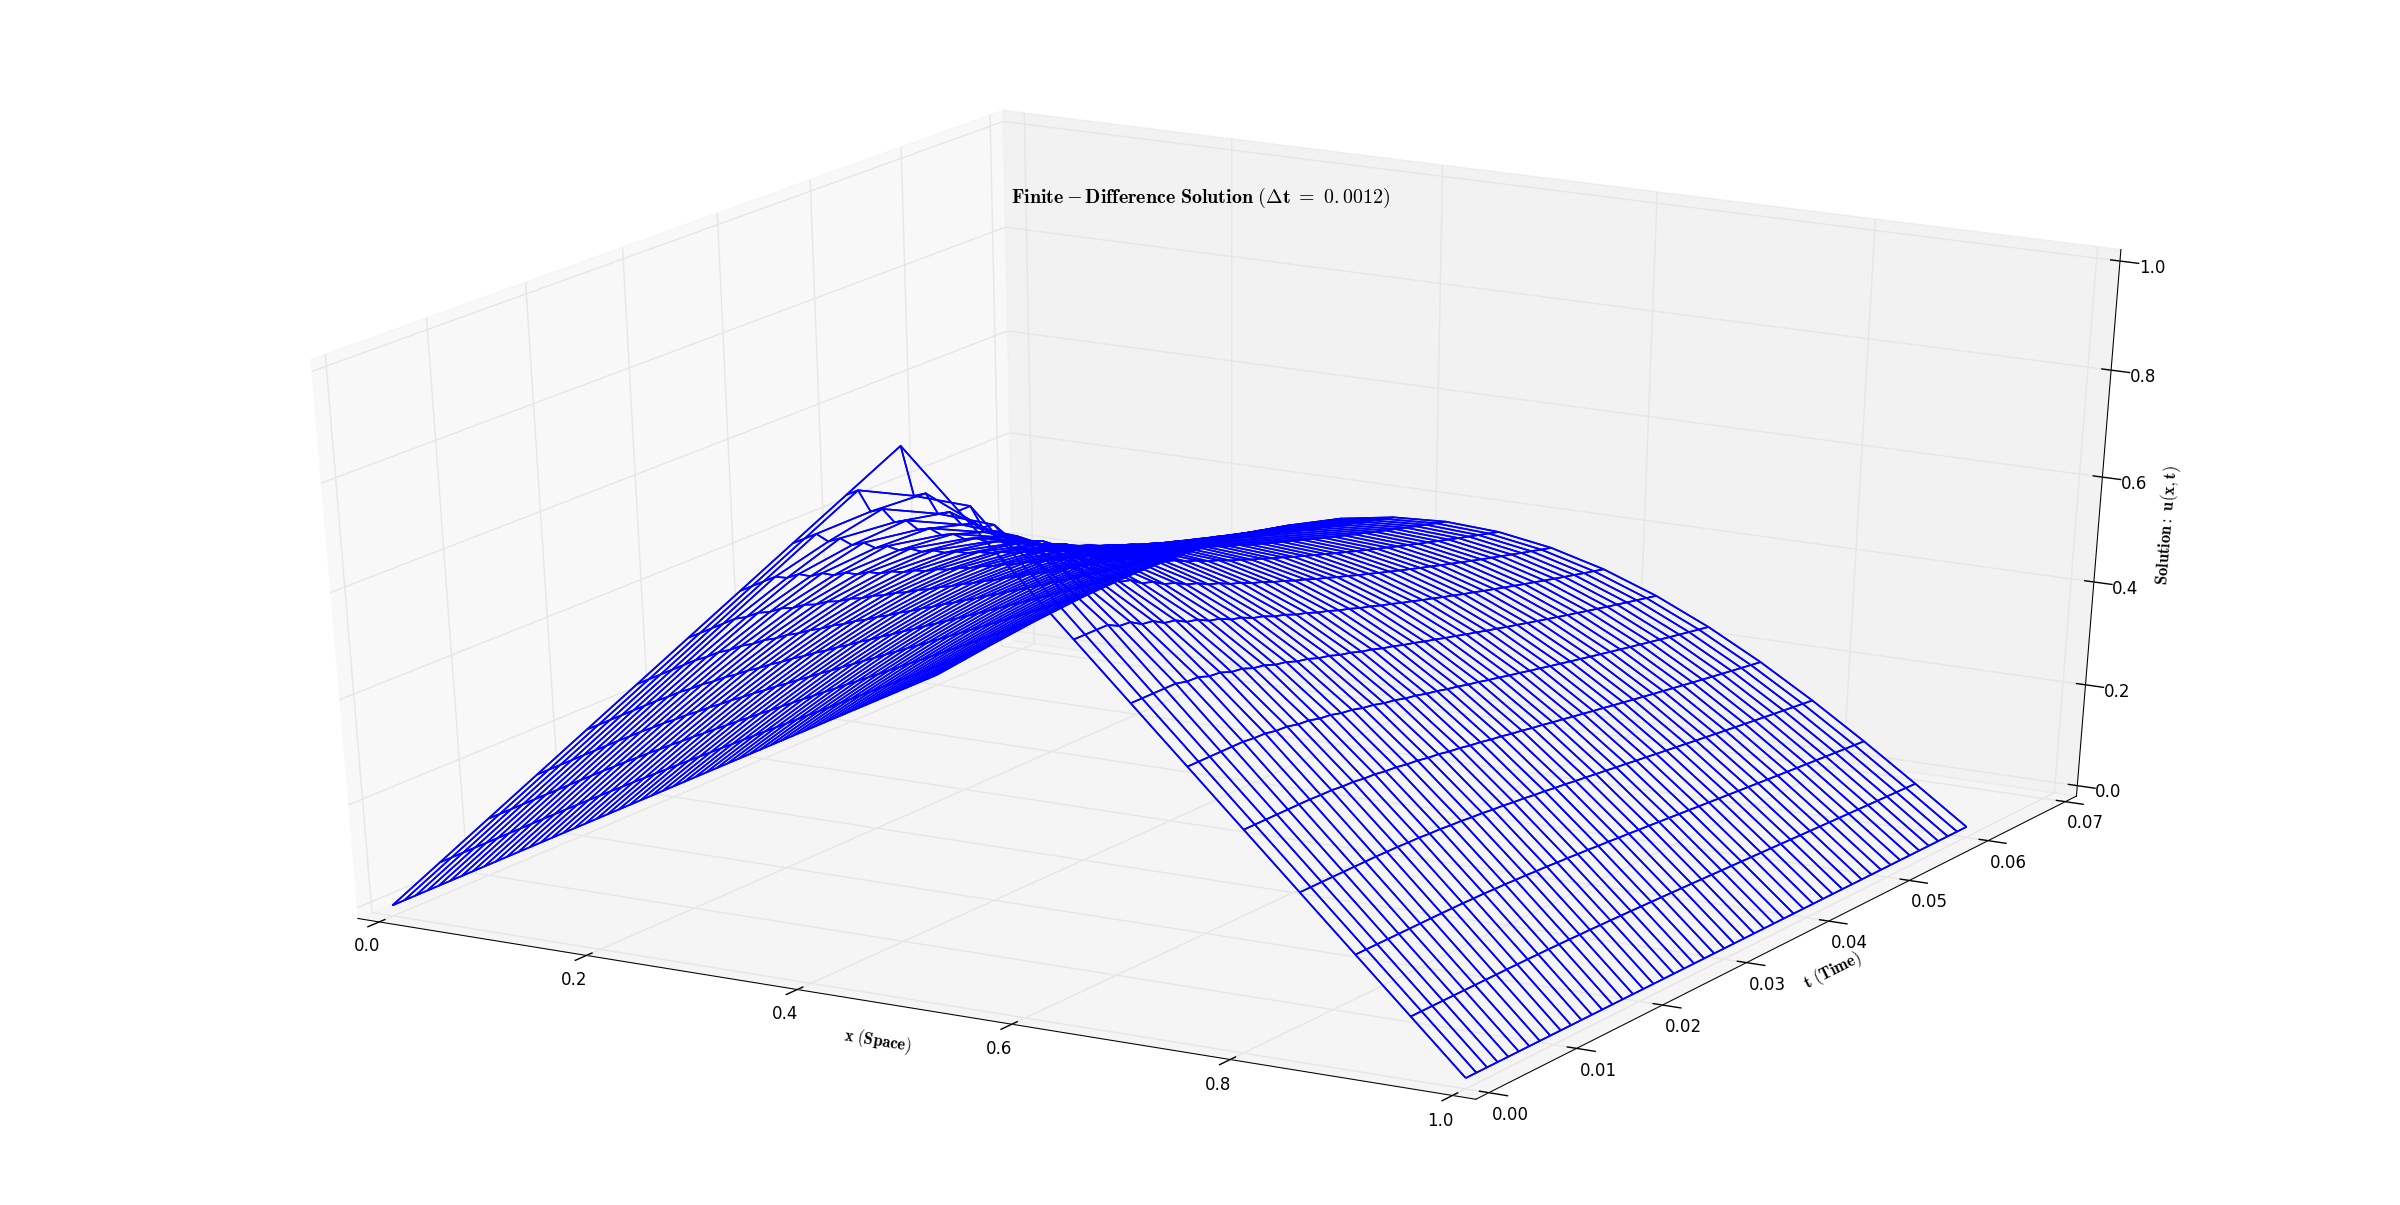
\includegraphics[width=7in]{Fig1}
\end{center} \hrule \newpage
\subsection*{(c): Newton's Method}
When solved with the Newton's method, the problem takes 5 iterations (quadratic convergence) to converge to the solution. The corresponding plot of the absolute error vs the number of iterations is given as shown:
\begin{center}
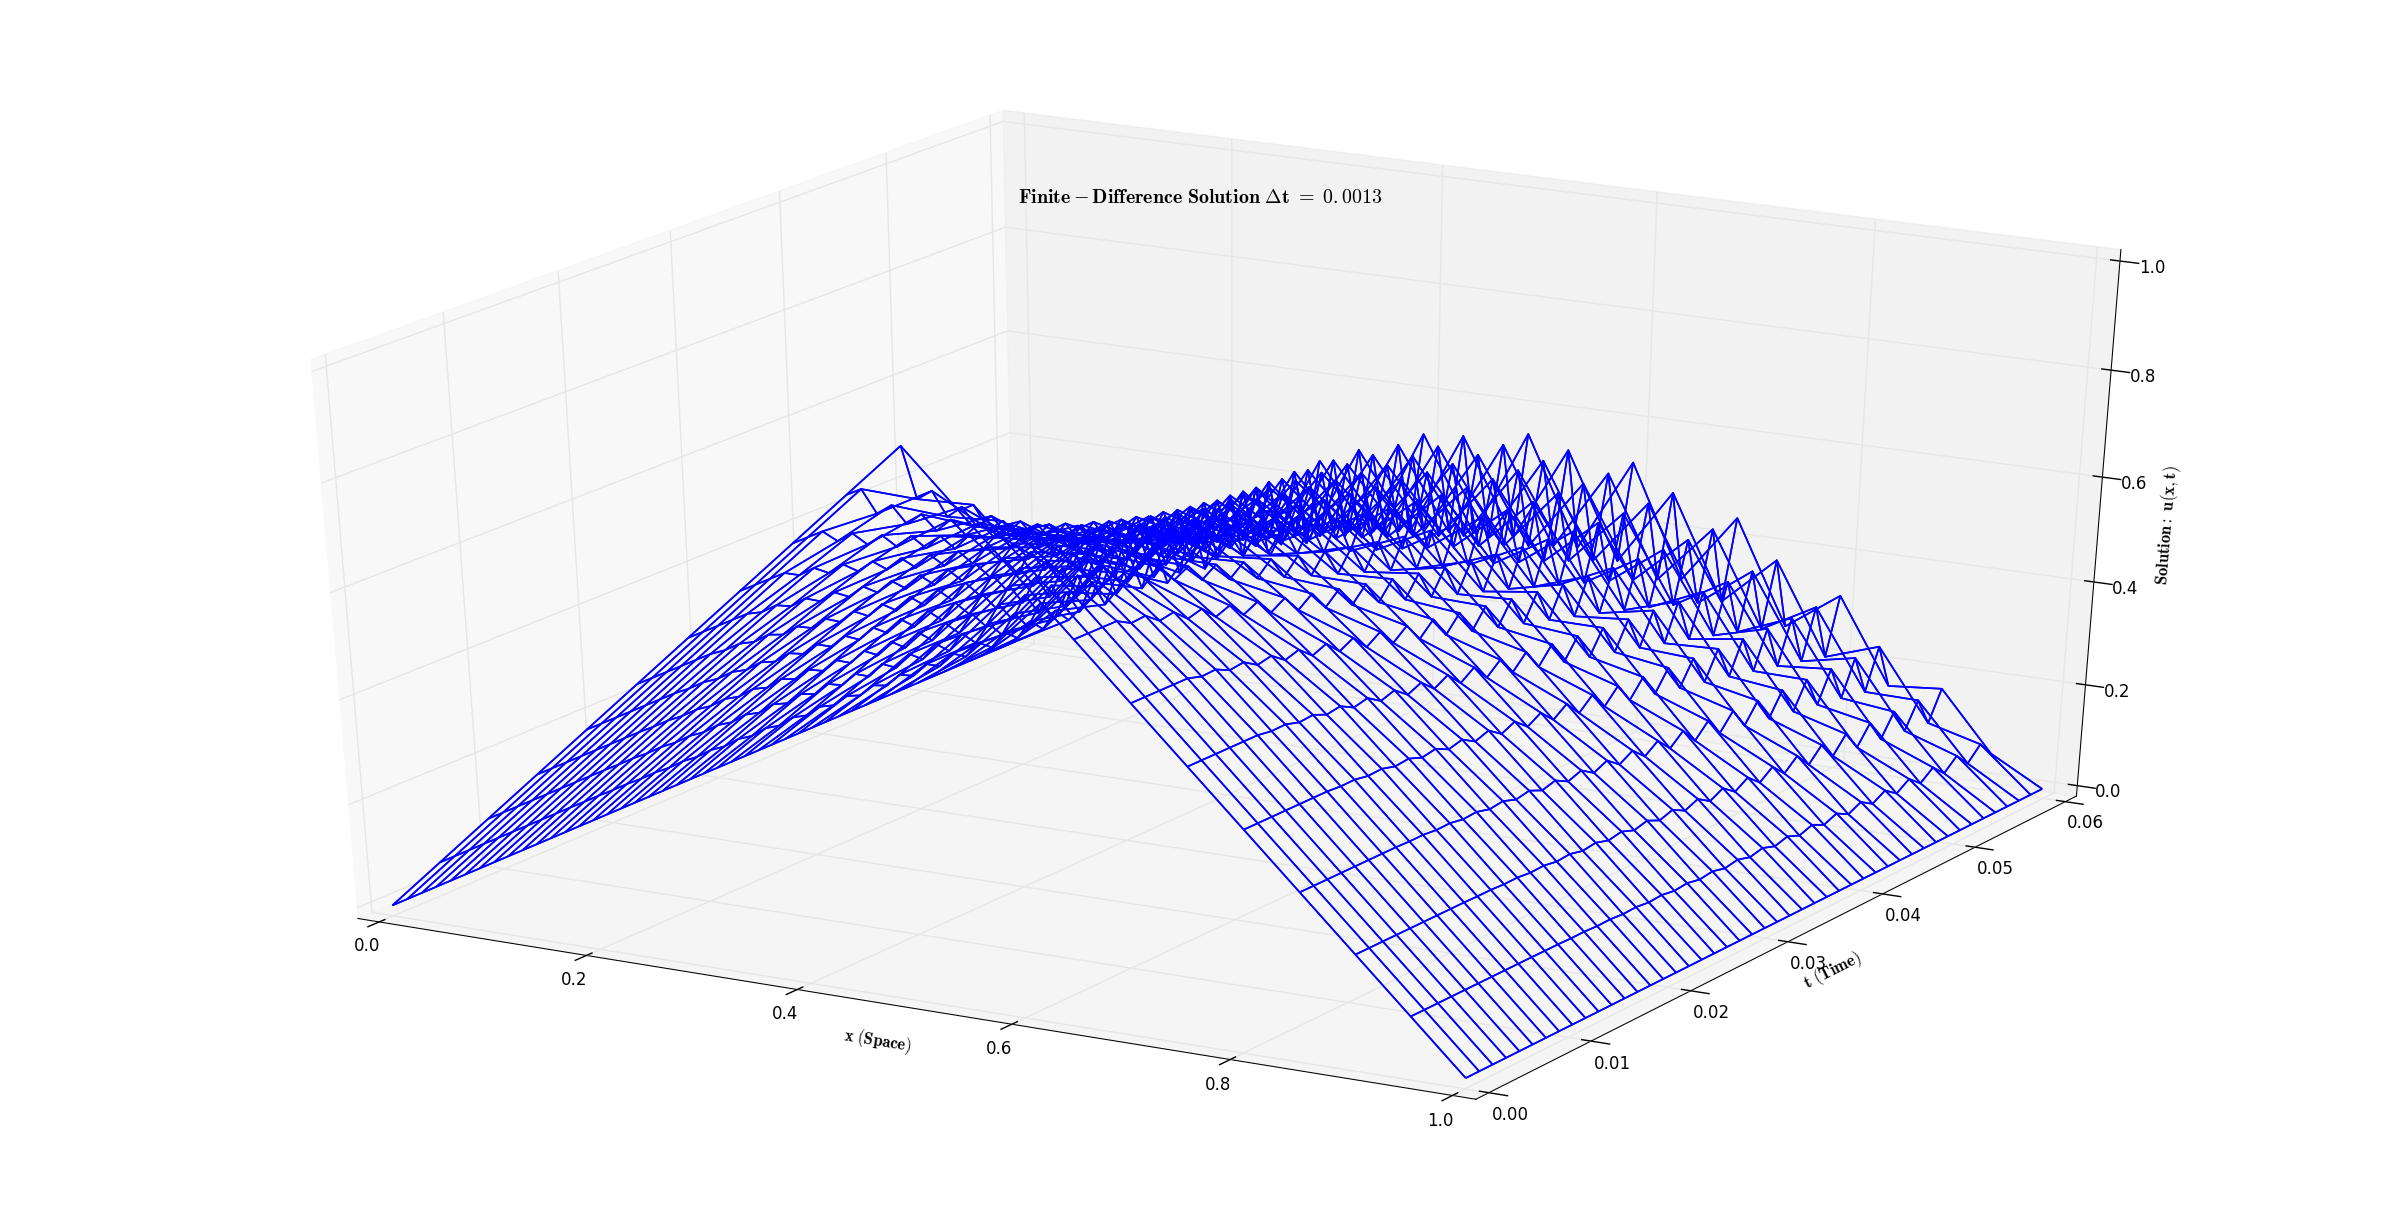
\includegraphics[width=7in]{Fig2}
\end{center} \hrule
\newpage\section*{Problem 5.24:}
The system of equations to be solved: 
\begin{align}
\begin{split}
w_1 + w_2 & = 2 \\
w_1x_1 + w_2x_2 & = 0 \\
w_1x^2_1+w_2x^2_2 & = \frac{2}{3} \\
w_1x^3_1+w_2x^3_2 & = 0
\end{split}
\label{524}
\end{align}
where $w_1$, $w_2$ denote the weights and $x_1$ and $x_2$ denote the corresponding gauss points. I use \emph{scipy.optimize.root} to determine the solution of the above nonlinear system of equations. The guesses used for the problem are as follows: 
\begin{align*}
\begin{Bmatrix}
w_1\\w_2\\x_1\\x_2
\end{Bmatrix}_{\rm trial}
=
\begin{Bmatrix}
1.0\\1.0\\0.577\\-0.577
\end{Bmatrix}
\end{align*}
which verifies the analytically the existing solution: 
\begin{align}
\begin{Bmatrix}
w_1\\w_2\\x_1\\x_2
\end{Bmatrix}_{\rm computed}
=
\begin{Bmatrix}
1.0\\1.0\\0.577\\-0.577
\end{Bmatrix}
\end{align}
Another guess 
\begin{align*}
\begin{Bmatrix}
w_1\\w_2\\x_1\\x_2
\end{Bmatrix}_{\rm trial}
=
\begin{Bmatrix}
1.0\\1.0\\0.0\\0.0
\end{Bmatrix}
\end{align*}
yields the following solution 
\begin{align*}
\begin{Bmatrix}
w_1\\w_2\\x_1\\x_2
\end{Bmatrix}_{\rm computed}
=
\begin{Bmatrix}
1.000001\\0.999999\\0.577\\-0.577
\end{Bmatrix}
\end{align*}
Several other perturbations result in very slight variation in the solution. Hence there is a single solution to the above system of nonlinear equations. It is, however, important to note that all the guesses which are considered here satisfy the first equation in (\ref{524}), atleast. A starting guess of $[0,0,0,0]'$ doesn't result in convergence and hence is avoided. \\ \hrule
\newpage\section*{Problem 8.6: }
The problem specifies to use an adaptive quadrature routine to compute the integral. For this, the library routine \emph{scipy.integrate.quad} is employed to compute the integral. The integral values obtained from the different methods are plotted below to compare and contrast: 
\subsection*{(a): Adaptive Quadrature} The plot below shows the computed integral values as a function of the parameter $k$
\begin{center}
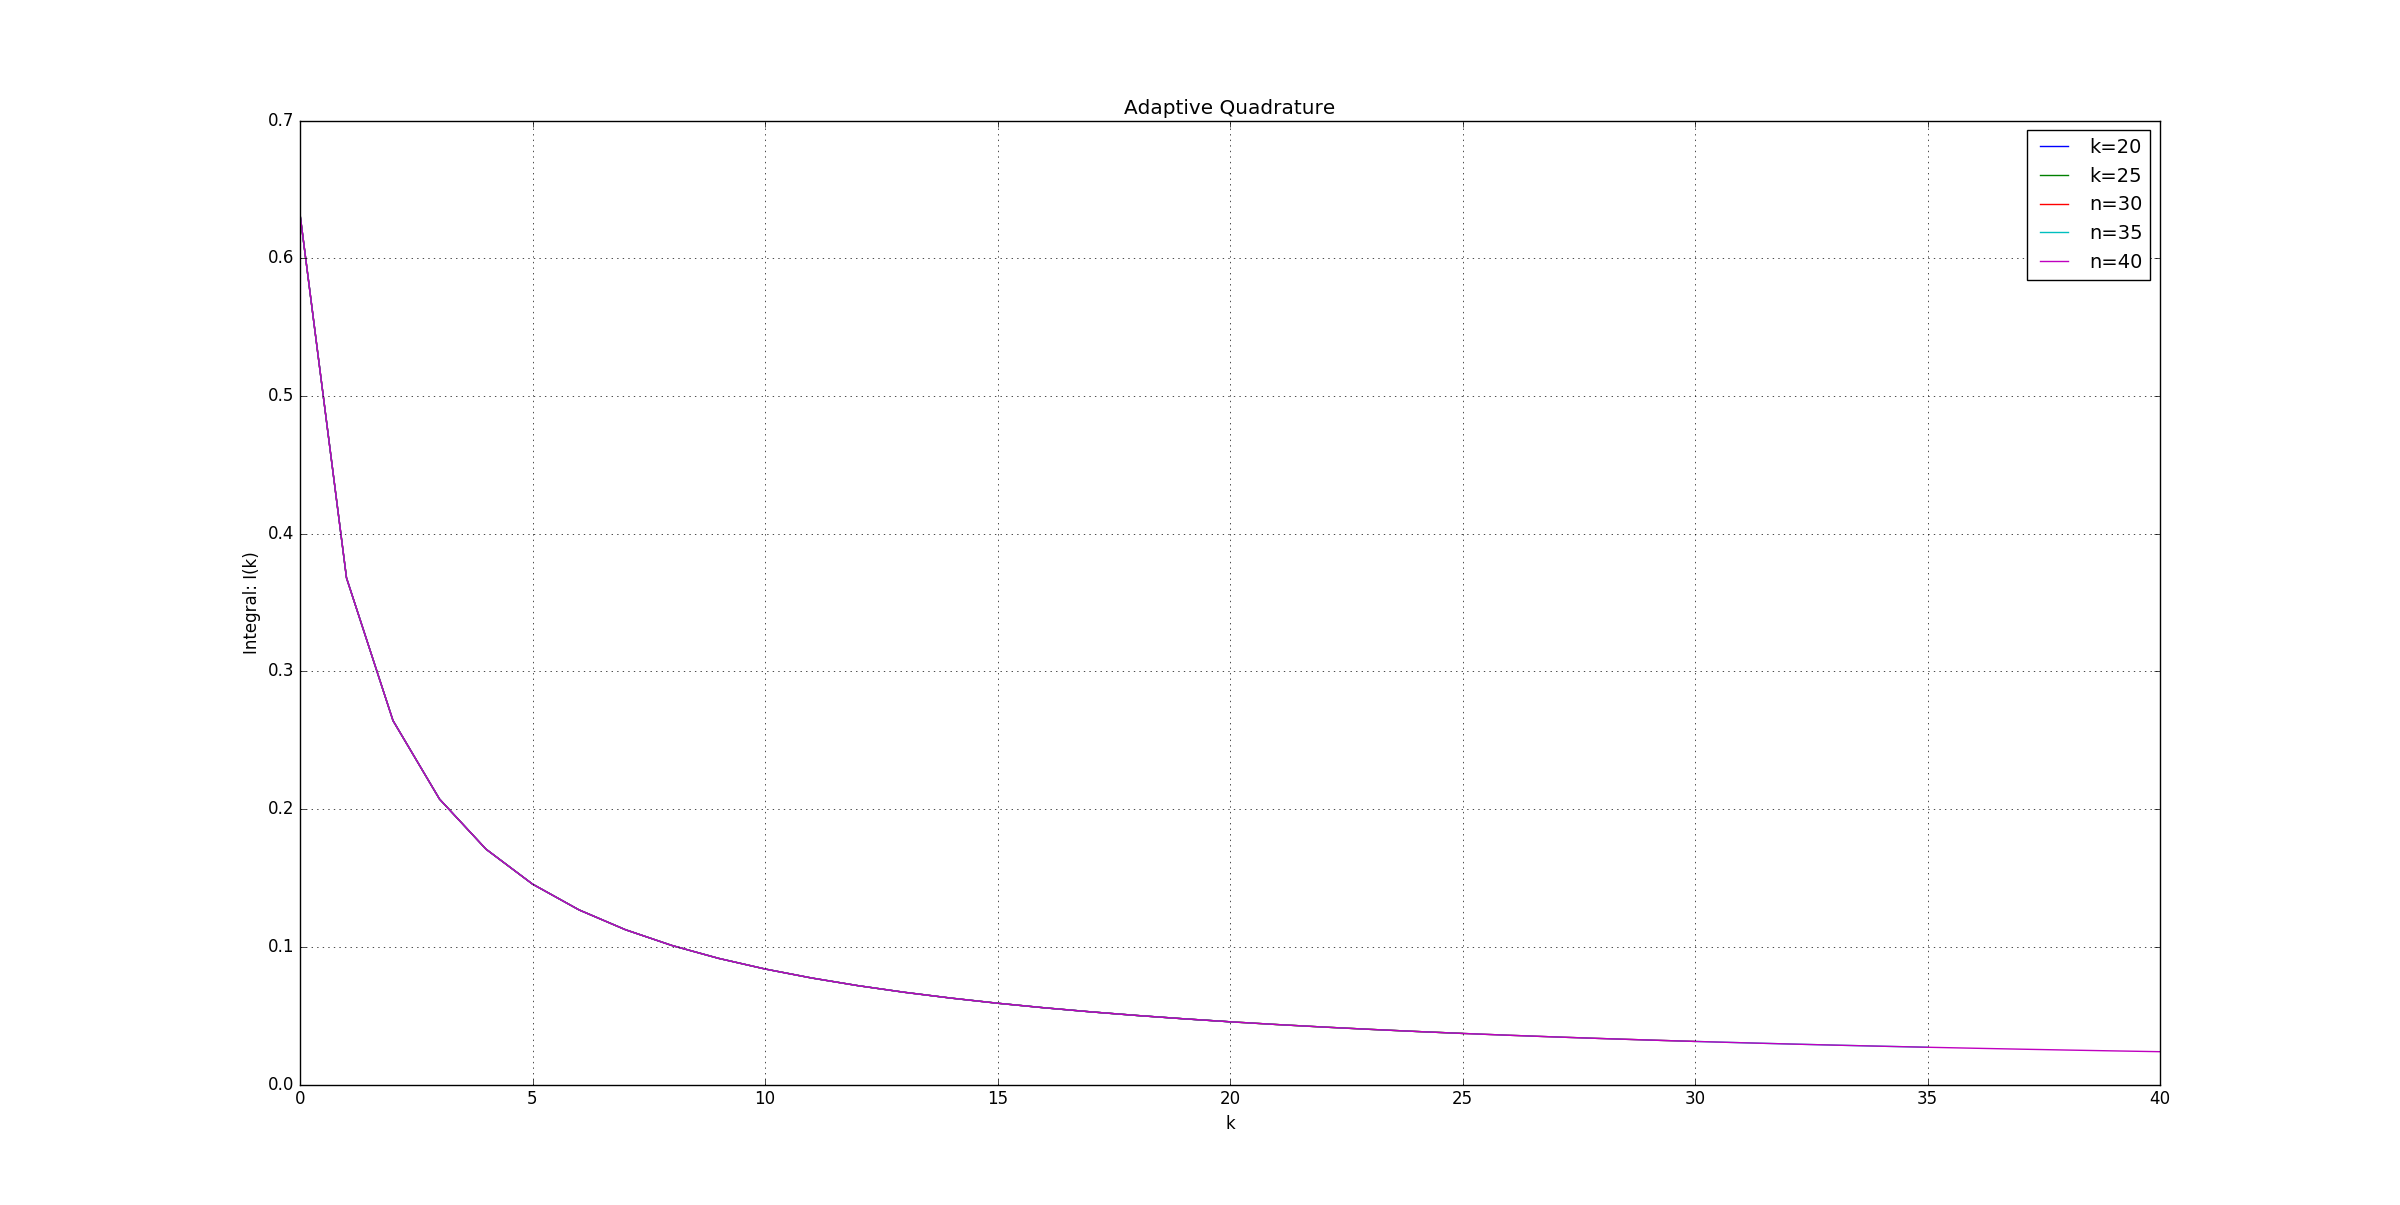
\includegraphics[width=7in, height=4.5in]{861}
\end{center}\hrule
\subsection*{(b): Forward Recurrence Relation}
The plot below shows the computed integral values as a function of the parameter $k$ using the forward recurrence relation. 
\begin{center}
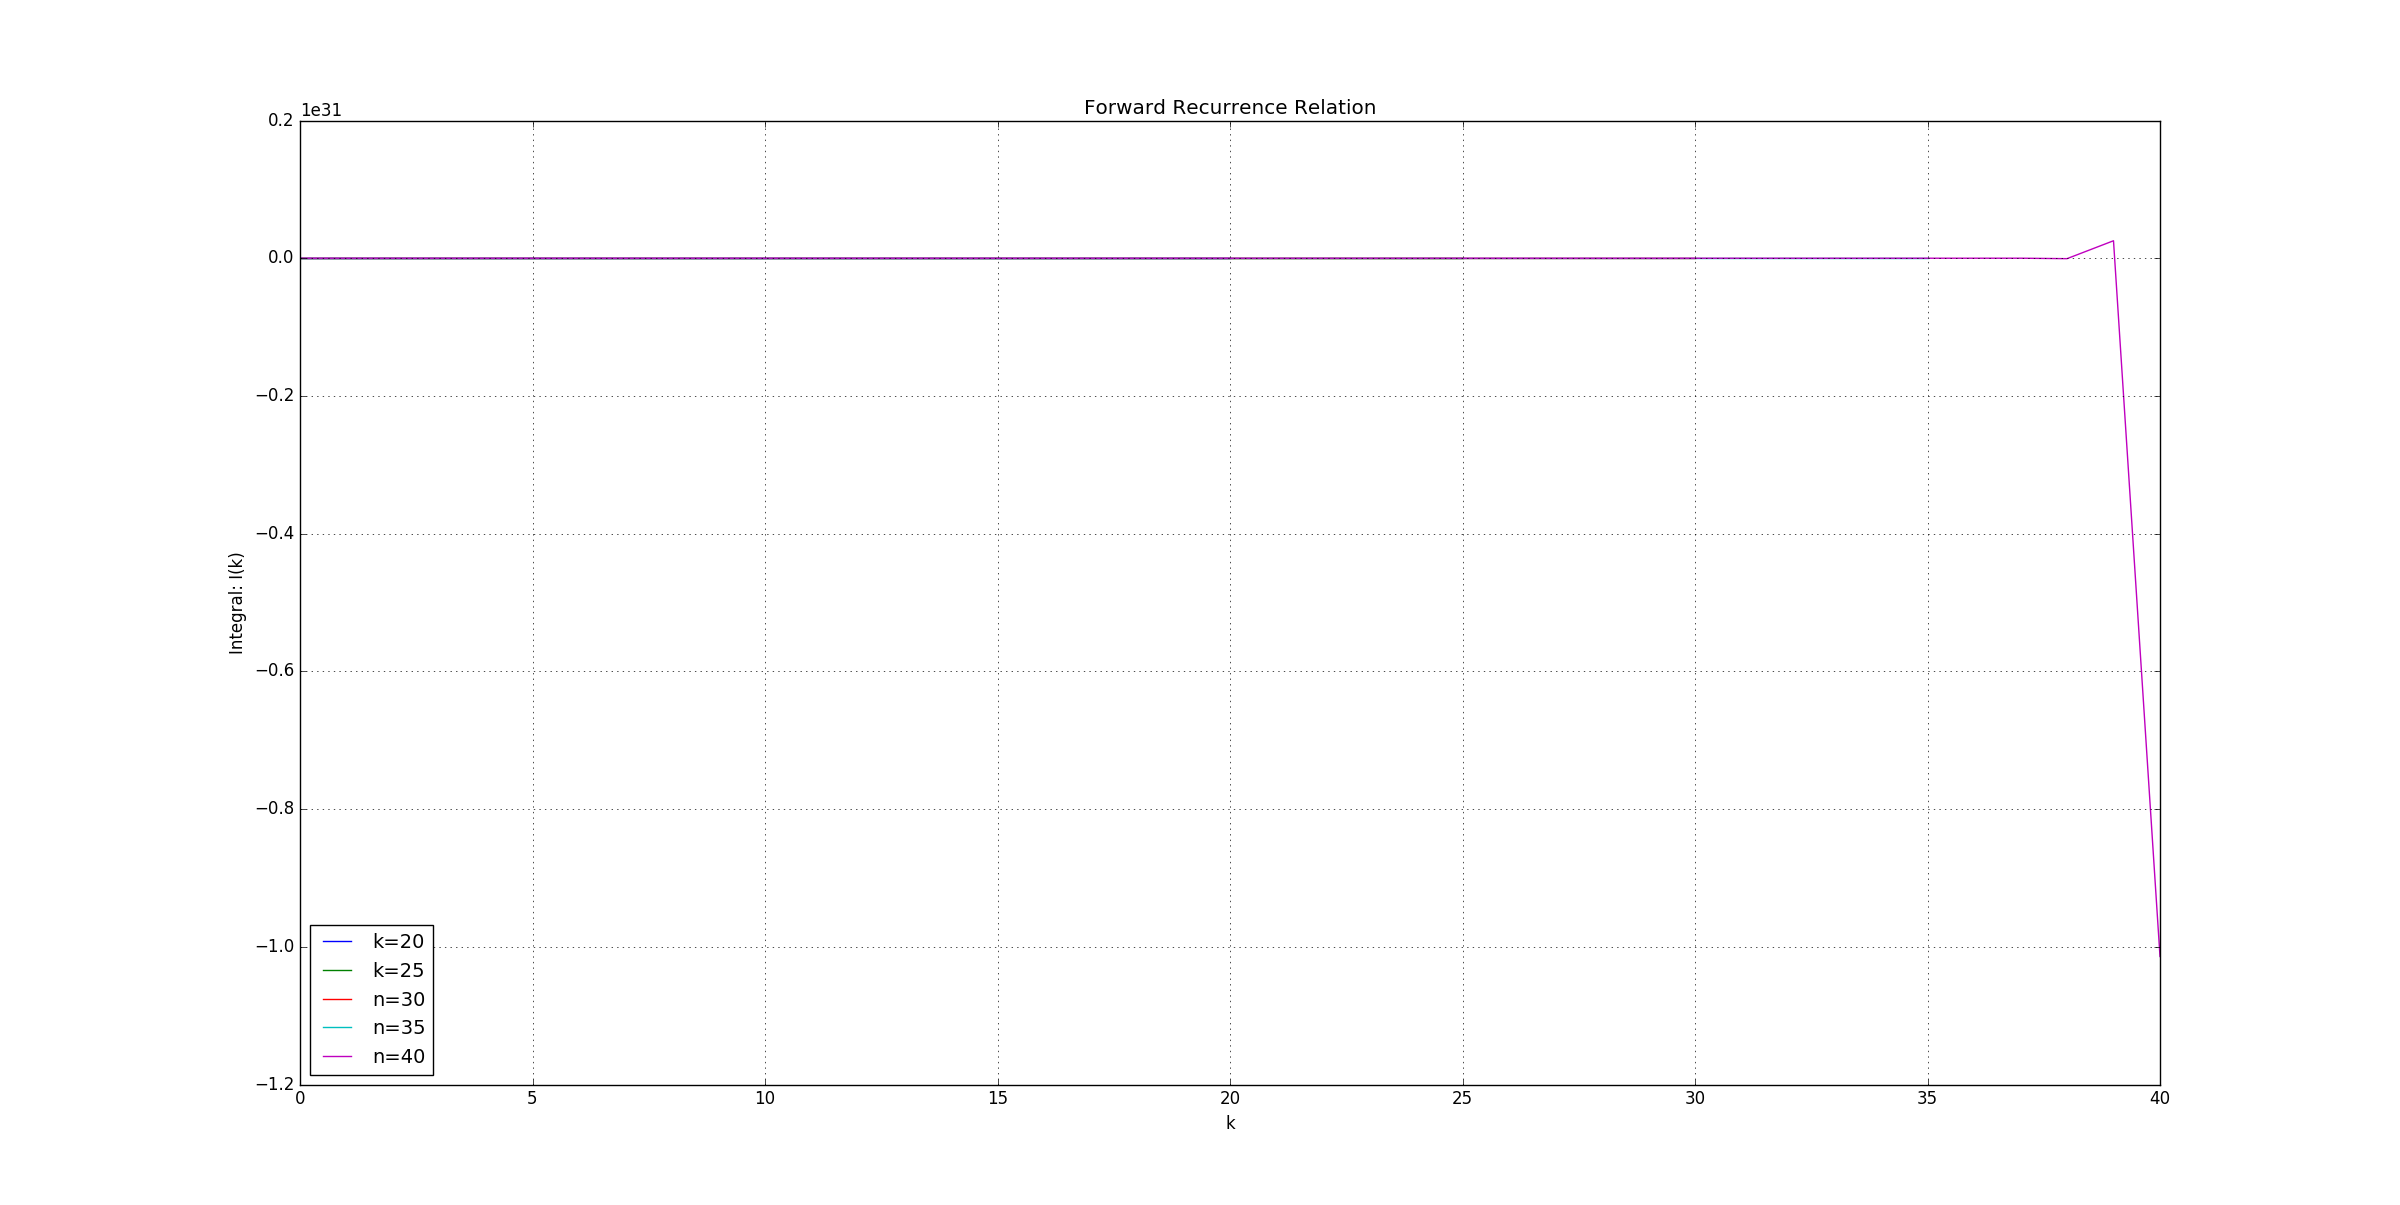
\includegraphics[width=7in, height=4.5in]{862}
\end{center}
It is plain from the above plot that the forward recurrence relation is increasingly unstable for larger values of the parameter $k$. \\ \hrule\newpage
\subsection*{(c): Backward Recurrence Relation}
The plot below shows the computed integral values as a function of the parameter $k$ using the backward recurrence relation. 
\begin{center}
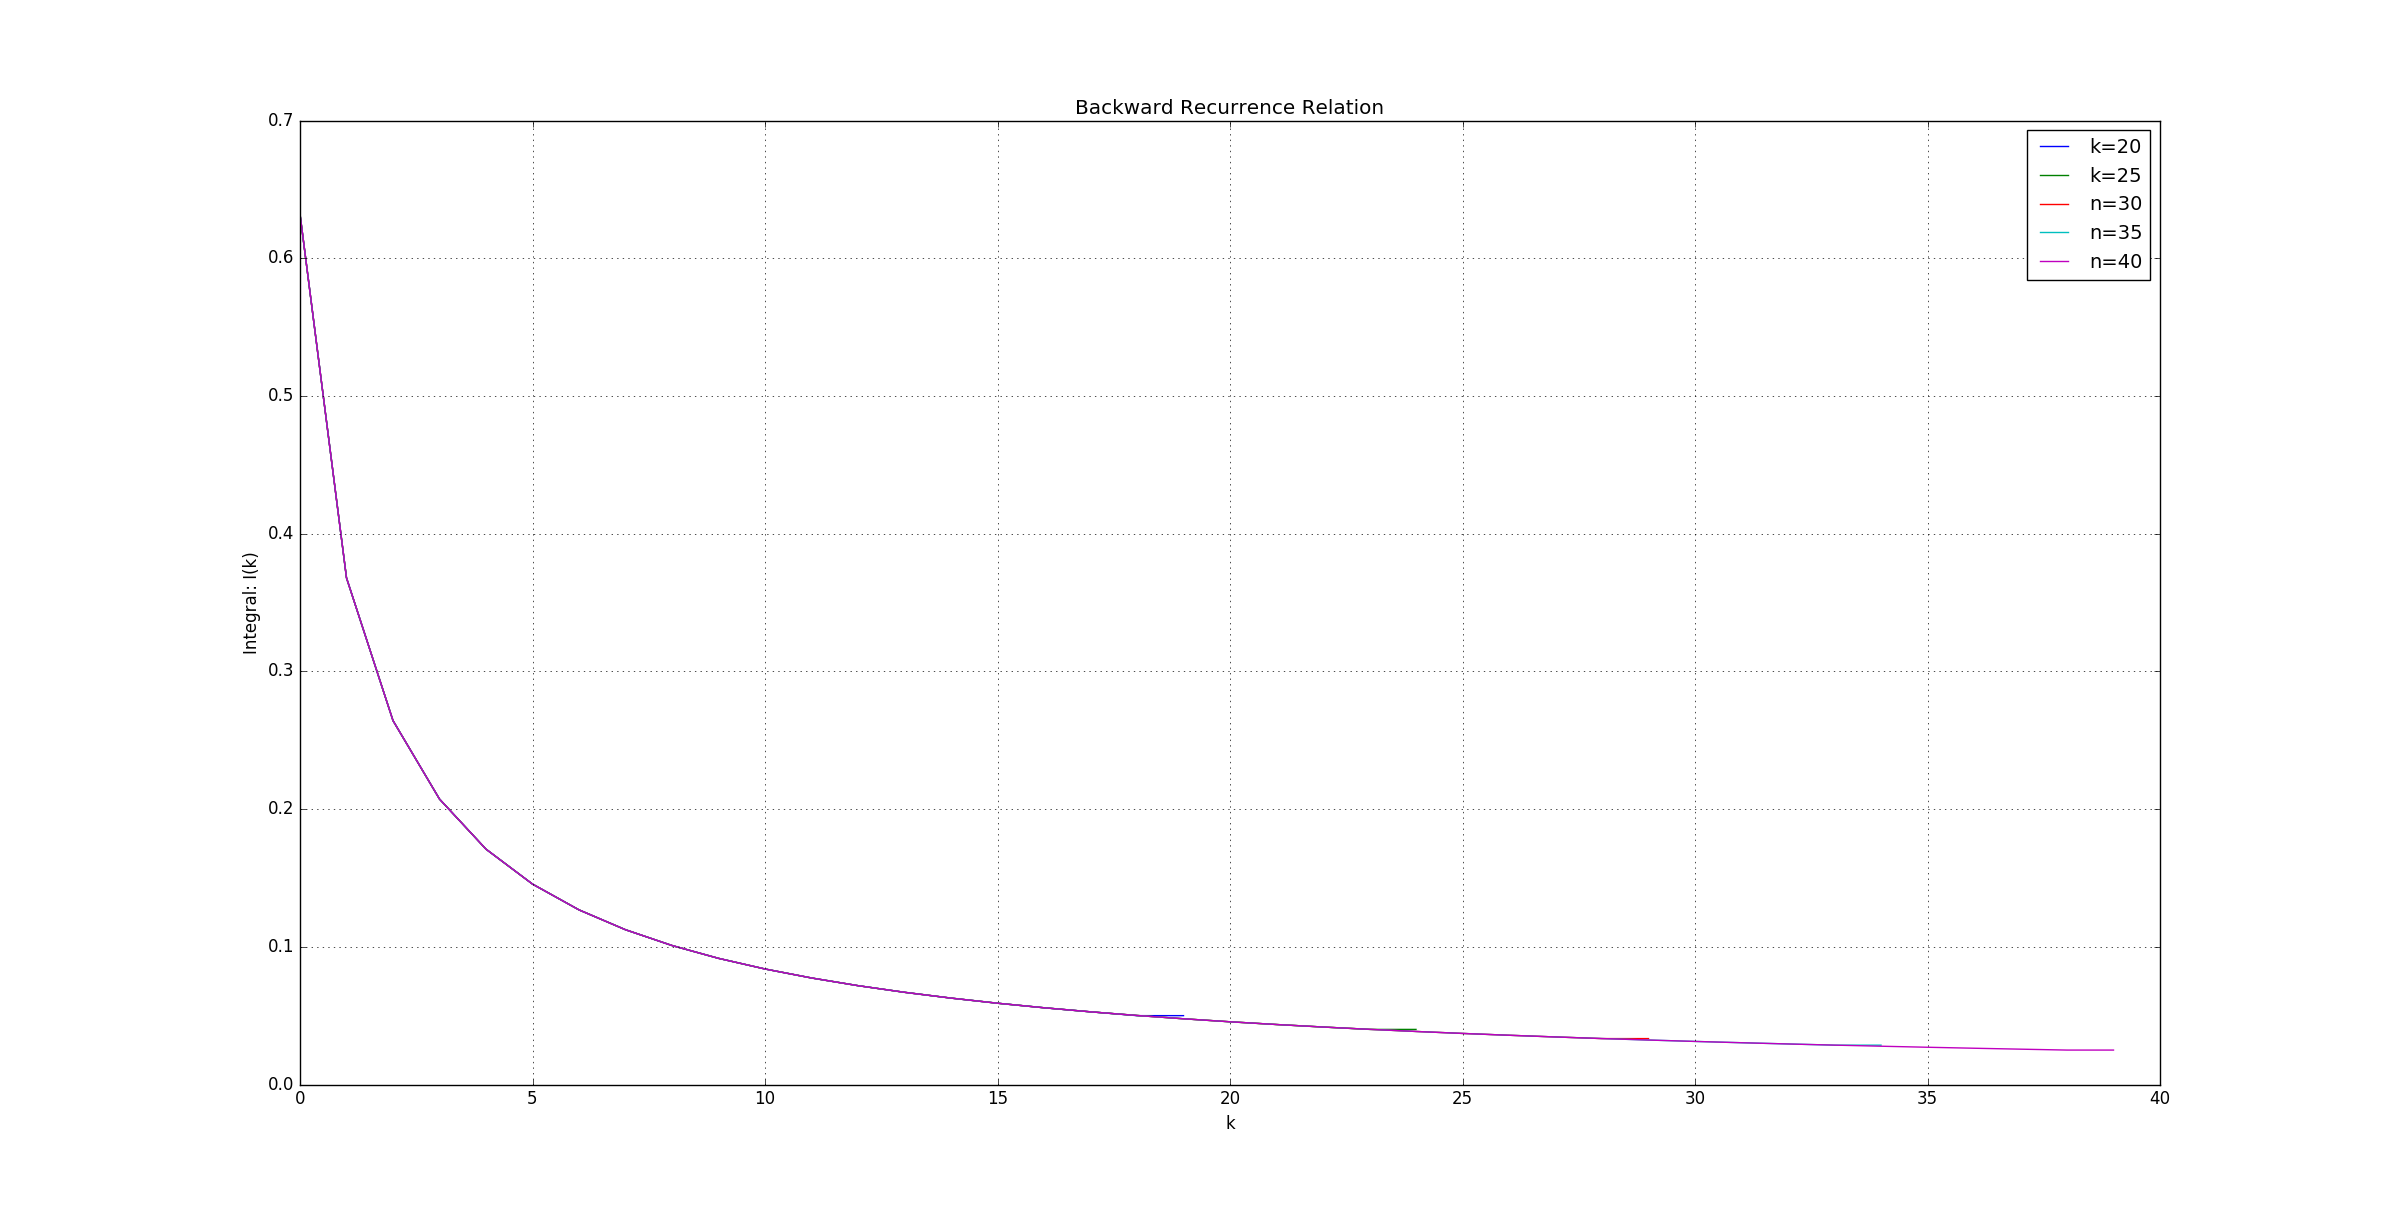
\includegraphics[width=7in, height=4.5in]{863}
\end{center}
The backward recurrence relation, unlike the forward recurrence relation, is much more stable for larger values of the parameter $k$.
\newpage\subsection*{(d): Comparison between Adaptive Quadrature and Backward Recurrence}
The plot below shows a comparative plot between the backward recurrence formula and the adaptive quadrature rule for $k=40$. We choose the maximum value of the parameter, among the set of values, in order to inspect the stability of the adaptive quadrature with respect to the backward recurrence formula and vice-versa. 
\begin{center}
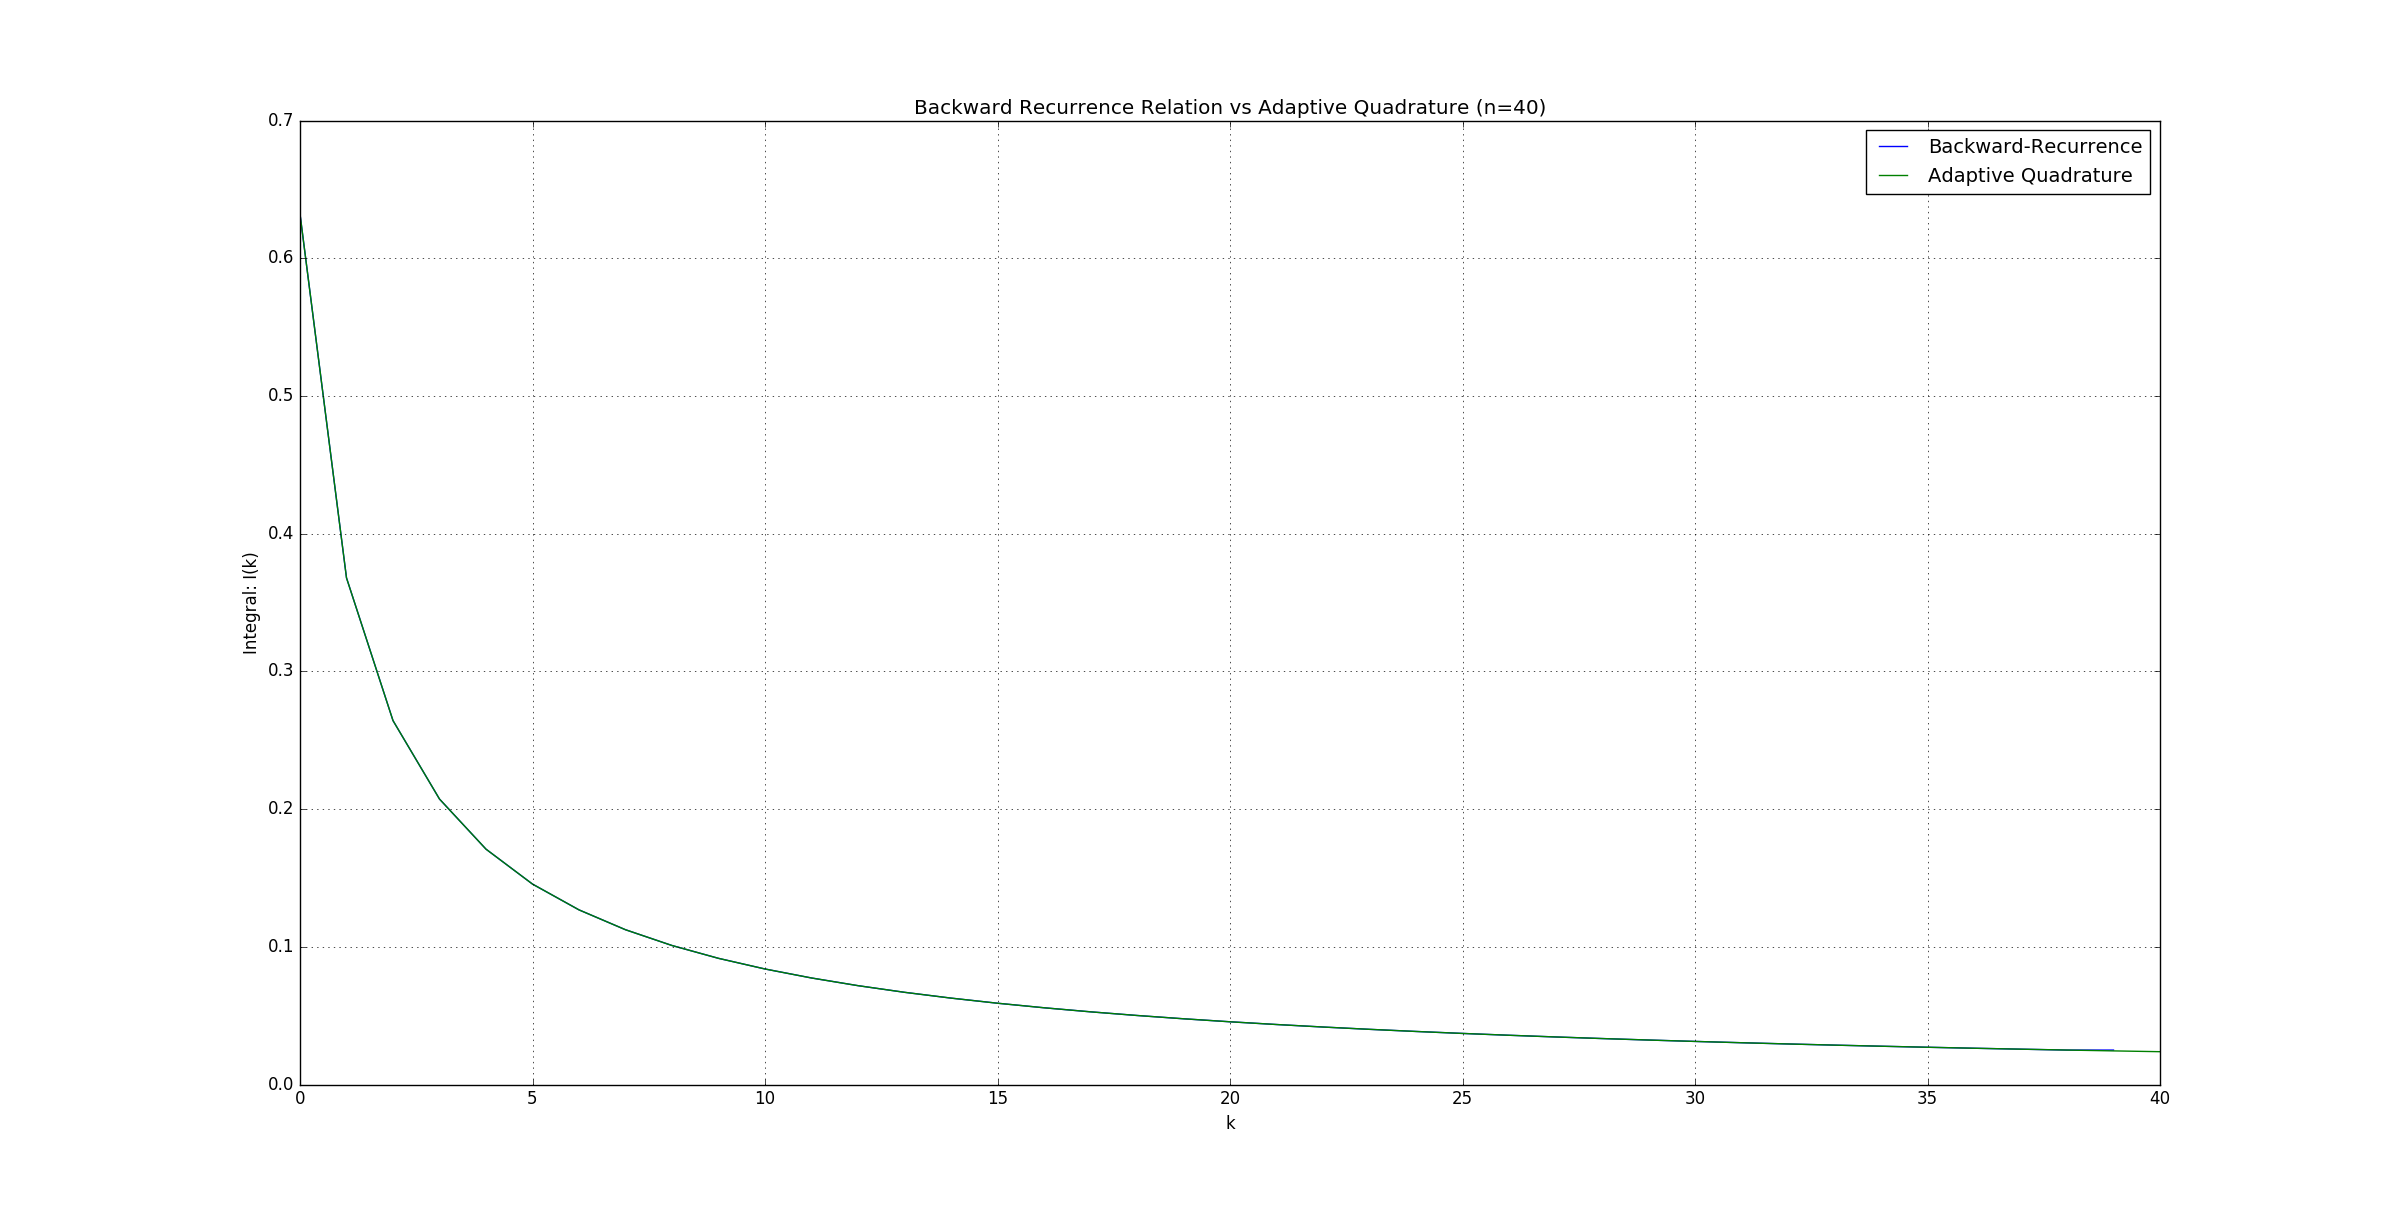
\includegraphics[width=7in, height=4.5in]{864}
\end{center}
\begin{itemize}
\item As a conclusive remark the forward recurrence relation is unstable for higher values of $k$, and the adaptive quadrature library routine and the backward recurrence formula are stable. 
\end{itemize}
\subsection*{(e): Comparison of Run-time}
\begin{itemize}
\item Since the backward and forward recurrence formula involve only substitution, they are ought to be faster than the adaptive quadrature routine, (\emph{quad}). However \emph{quad} is more accurate as compared to both of these.
\item The Backward recurrence formula assumes the value is equal to zero for a sufficiently large n and then proceeds in a backward manner to calculate. Hence there is no discretization error (which is incurred in case of the forward recurrence formula).
\end{itemize} \hrule
\newpage\section*{Problem 8.10: Gamma Function}
The given function to be integrated is: 
\begin{align*}
\Gamma(x)
=
\int_{0}^\infty
t^{x-1}
e^{-t}\ dt \ \ ; \ \ \ \ \ \ \ \ x > 0
\end{align*}
\subsection*{(a): Composite Quadrature Rule - Truncated interval}
For Composite-Quadrature rule, we choose the library routine \emph{scipy.integrate.simps} to compute the integral. The limit of integration imposed on the integration parameter $t$ is $(0,10^6)$ instead of the infinite integral, thereby using a truncated limit for the integral. The limit of integration which is used in this case, is determined after succesive trials with different upper limits, thereby making consideration for accuracy and runtime. 
\subsection*{(b): Adaptive Quadrature Rule - Truncated interval }
In this case we use the truncated interval to compute the integral and corresponding values are later plotted. It is observed that for the chosen truncation limit, the integral is approximated well by the truncated limits as opposed to the infinite integration limit. 
\subsection*{(c): Adaptive Quadrature - Infinite Interval}
The corresponding infinite integral is plotted below
\subsection*{(d): Gauss-Laguerre Quadrature - Degree (101) }
The Gauss-Laguerre Quadrature is better than the Simpson's rule for integration but is worse, in accuracy, than the Adaptive Quadrature. The corresponding plot (with all the methods) is attached below: 
\subsection*{Comments: }
The following observations can be made: 
\begin{itemize}
\item The Simpson's rule incurs the largest error among all the methods. 
\item The Adaptive Quadrature is very accurate even when evaluating the infinite integral. 
\item The Gauss-Laguerre Quadrature, for the chosen degree to calculate the infinite integral, is more accurate than the Simpson's rule (Composite Quadrature) but is less accurate than the adaptive quadrature.
\end{itemize}
\begin{center}
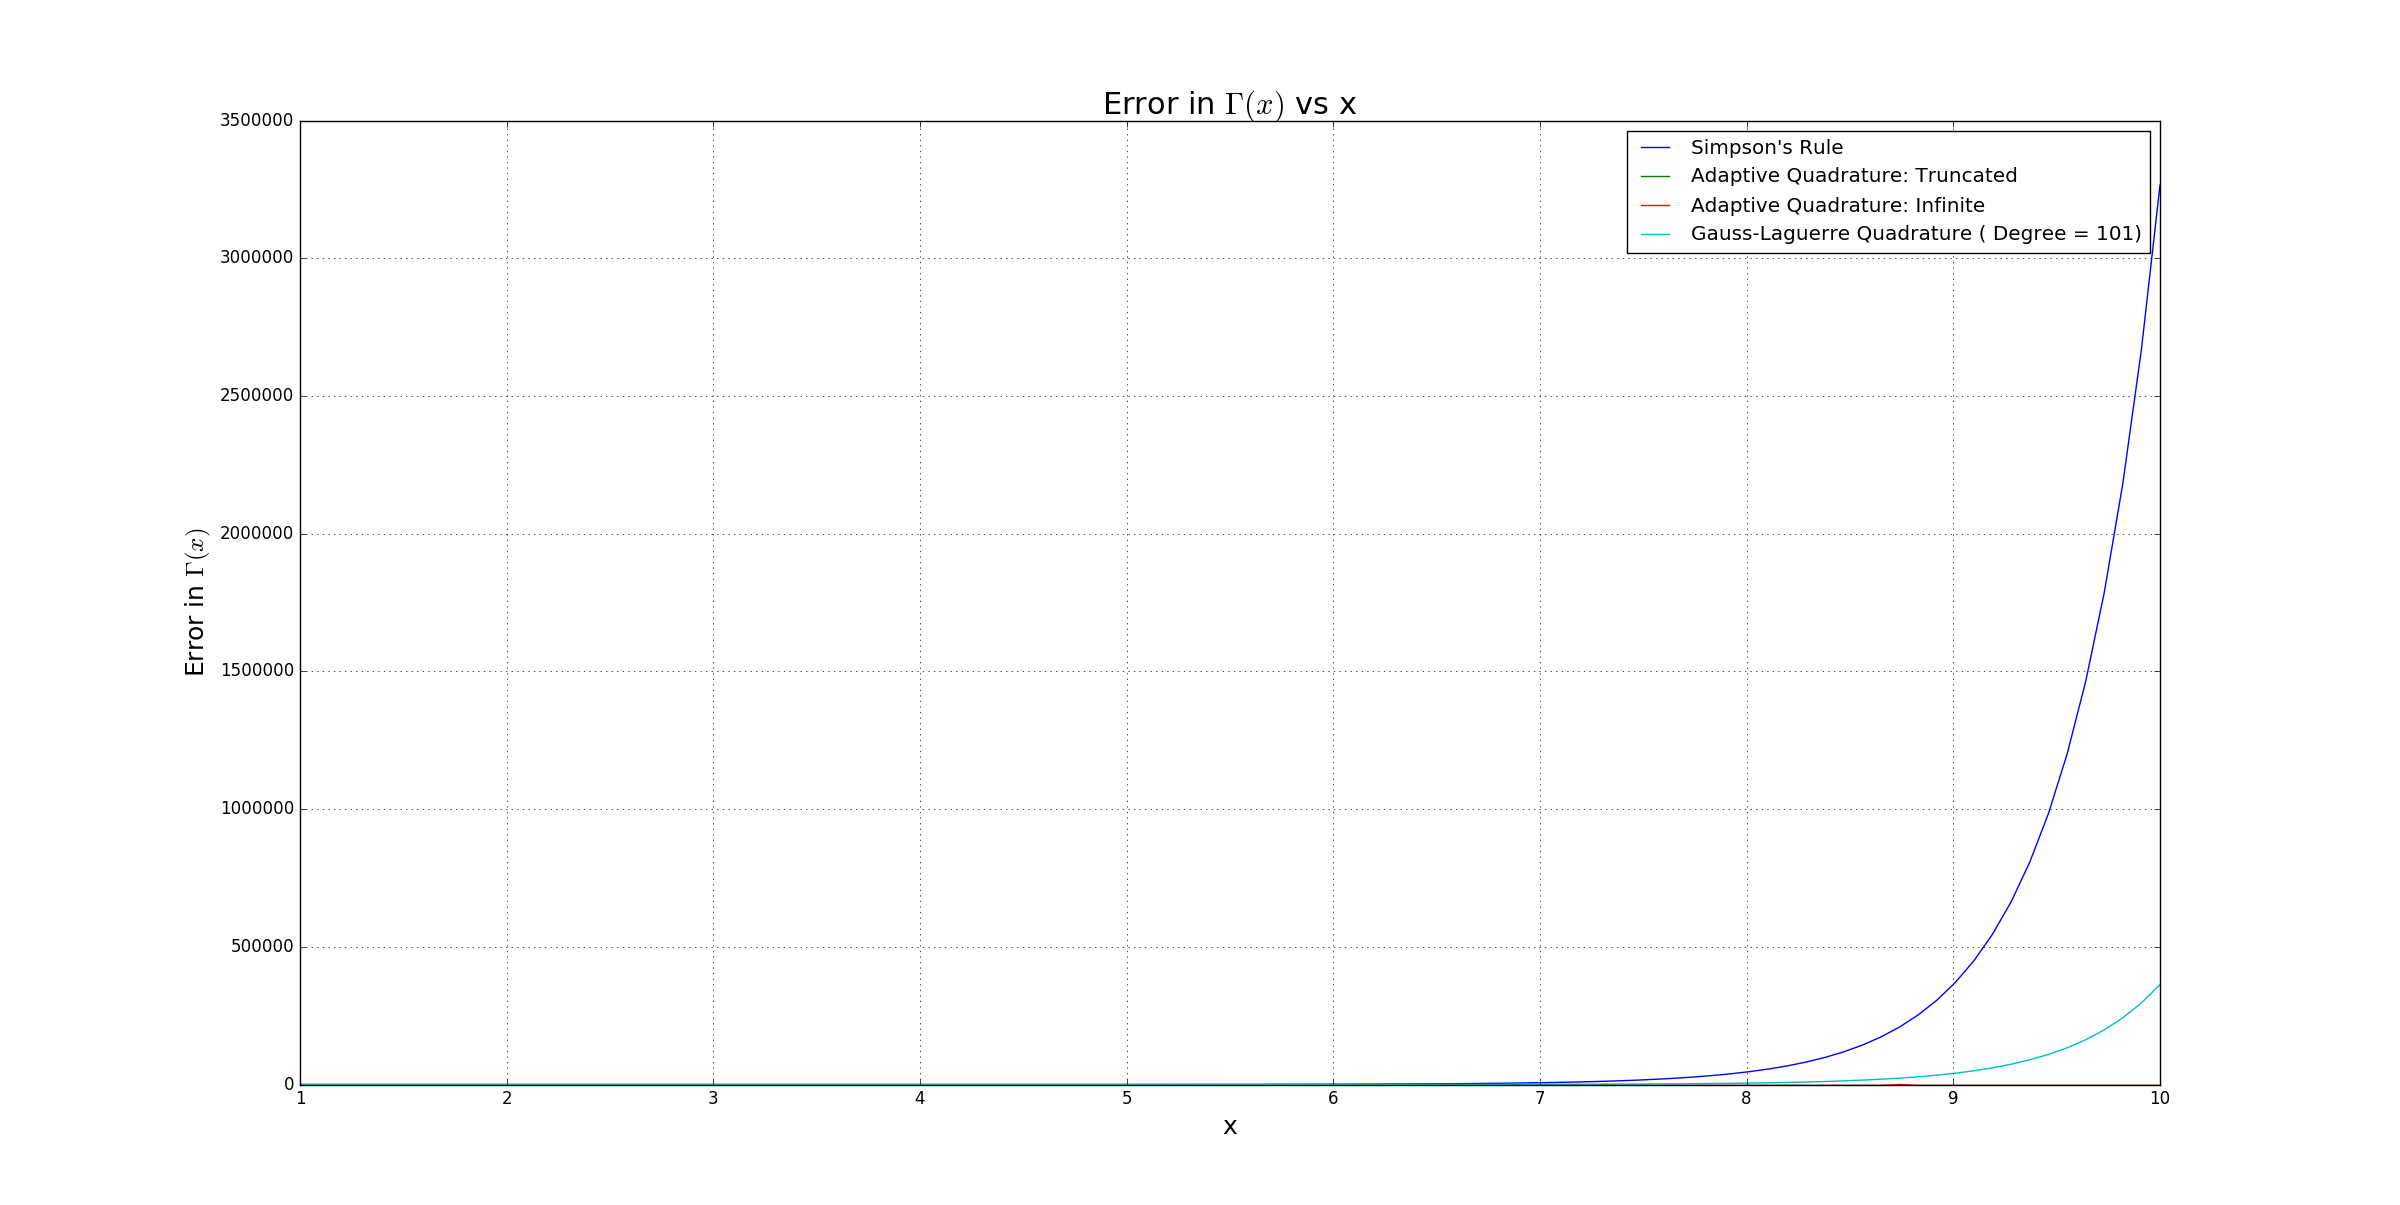
\includegraphics[width = 7in, height = 5in]{810}
\end{center}\hrule
\newpage\section*{Problem 8.17: Integral Equation: }
The integral equation to be solved: 
\begin{align*}
\int_{0}^1
{\left( 
s^2+t^2
\right)}^{1/2}\ u(t)\ dt = \frac{{\left( s^2+1\right)}^{3/2}-s^3}{3}
\end{align*}
The corresponding true solution is given by: 
\begin{align*}
u(t) = t
\end{align*}
\subsection*{Note: }
It is noted that all the plots below are given for $n=3,5,7,9,11,15$
\subsection*{(a): Gaussian-Elimination with Partial Pivoting}
Now we use the Simpson's rule (Composite Quadrature) to formulate the linear system which is then solved using the process of Gaussian-elimination with partial pivoting. The corresponding results obtained are as follows: 
\begin{center}
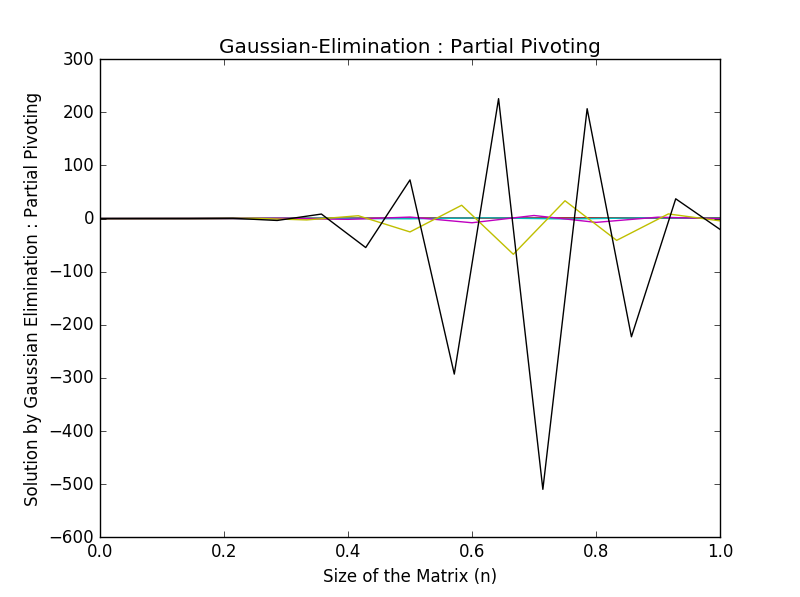
\includegraphics[scale=0.7]{GEPP}
\end{center}\hrule
\newpage\subsection*{(b): Condition Number}
The condition number of the matrix ($\bf A$) as a function of ($n$) is plotted below. It can be seen that the condition number of the matrix $\bf A$, increases with ($\bf n$). Increasing the size of the matrix (n) makes the matrix increasingly ill-conditioned. 
\begin{center}
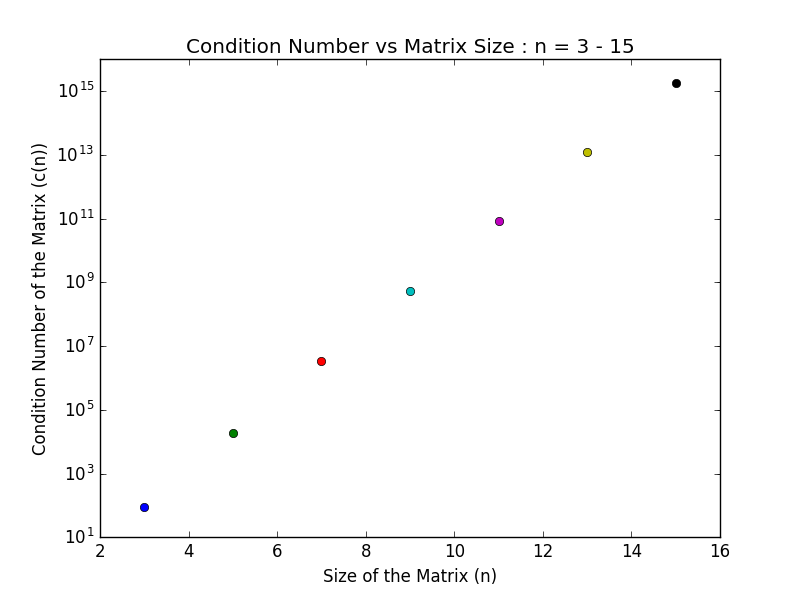
\includegraphics[scale=0.7]{CN}
\end{center}\hrule
\newpage\subsection*{(c): SVD} 
Here, in order to ignore the small singular values, through SVD, the criteria that is employed, to ignore a particular Singular values, is if the ratio of the maximum and the minimum singular values of the matrix. The corresponding plot is attached below: 
\begin{center}
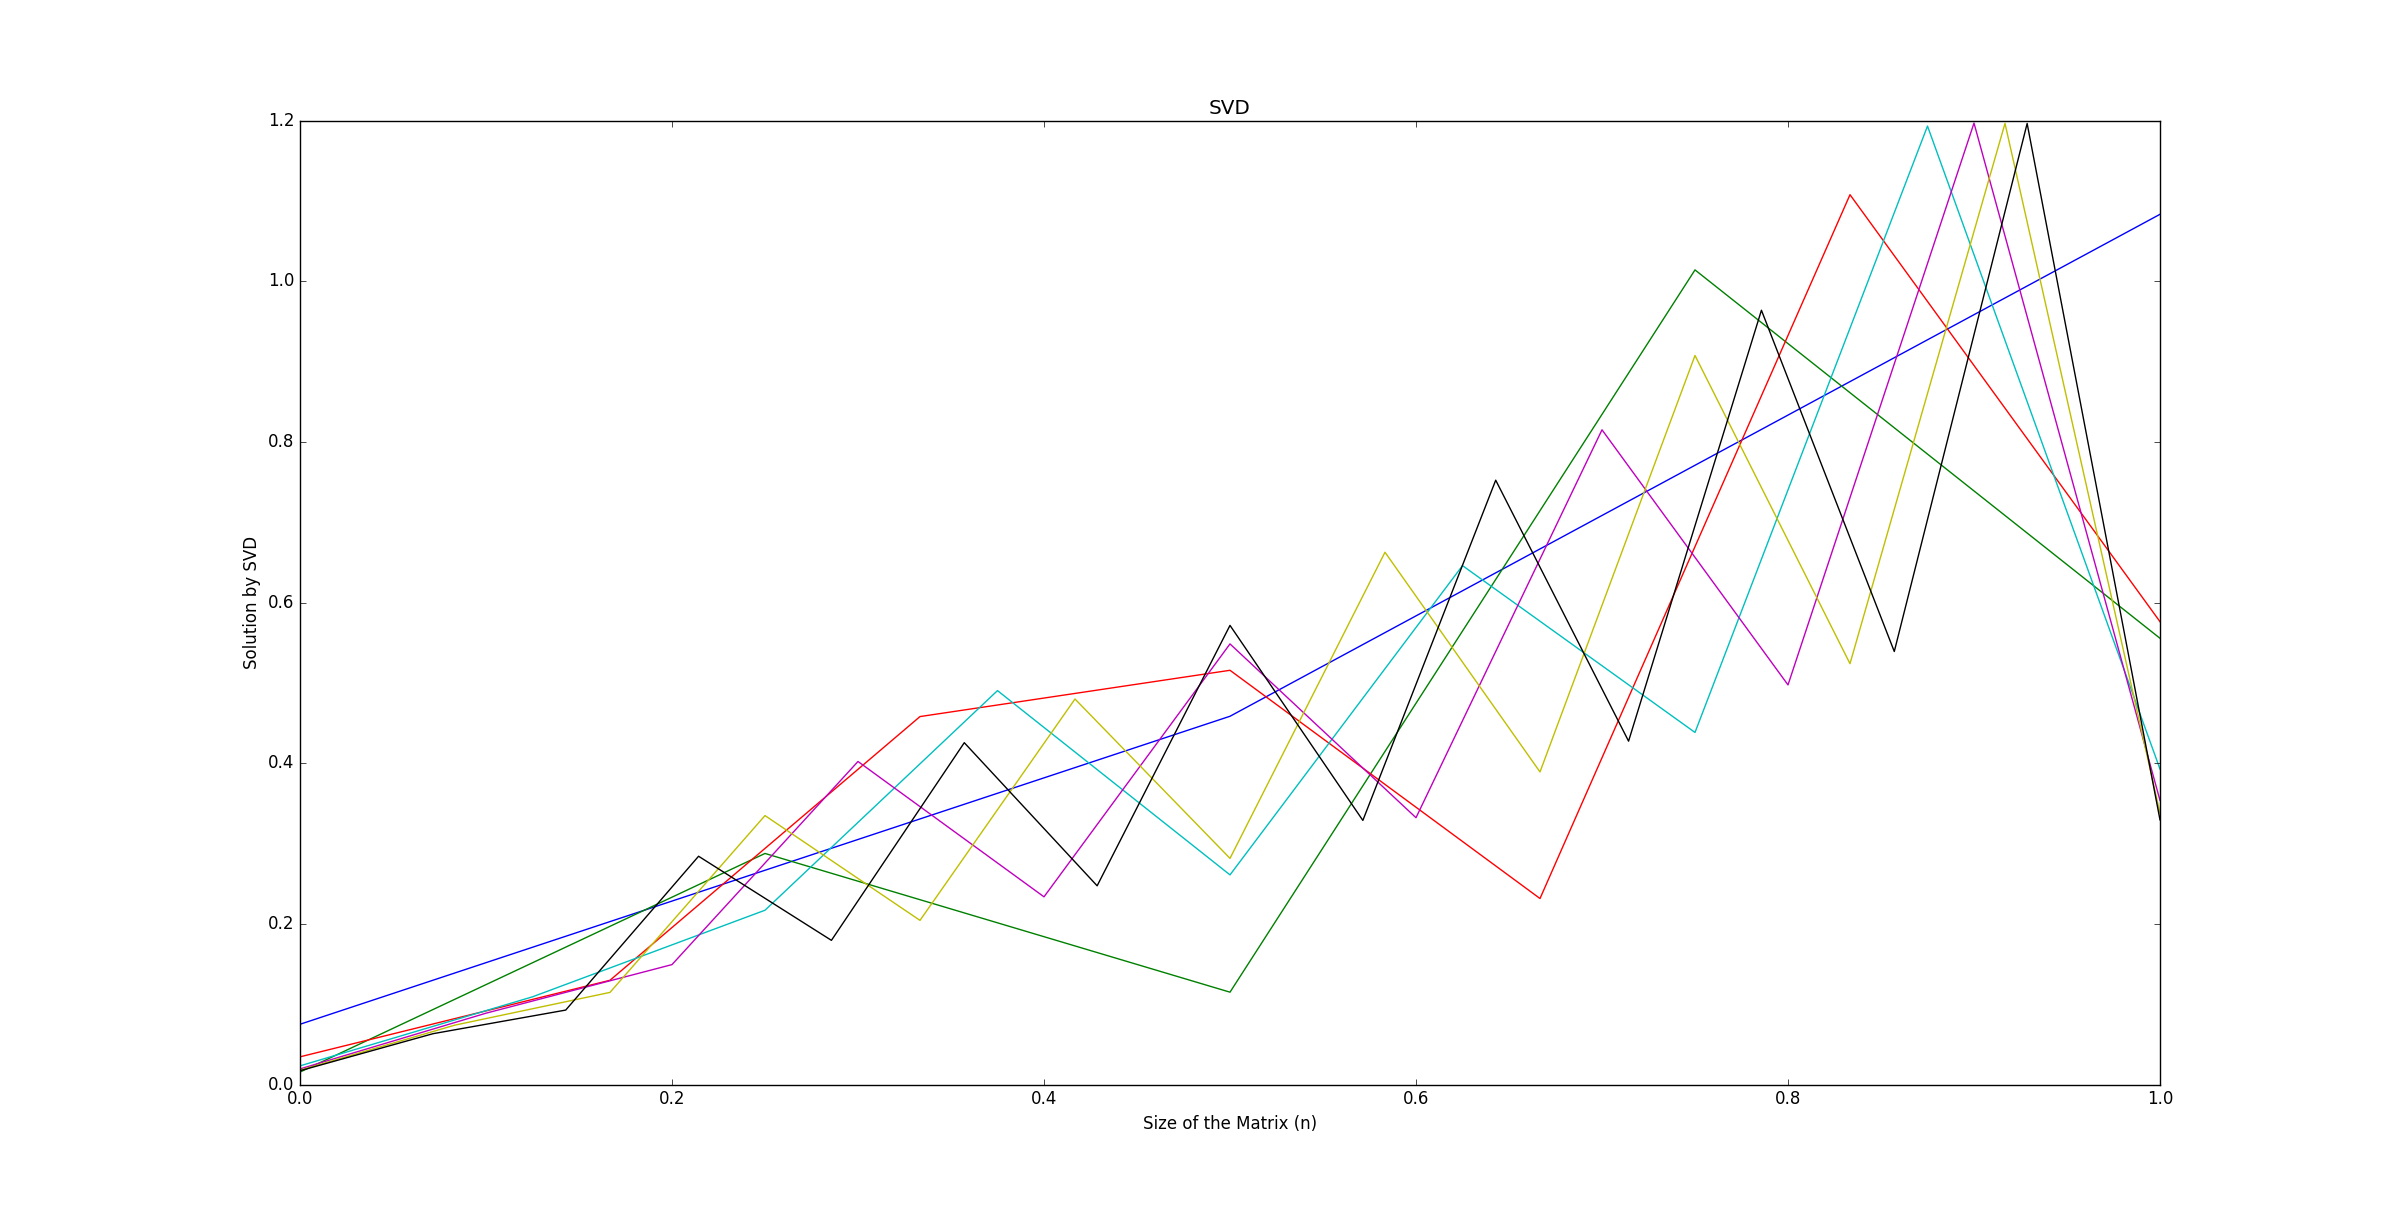
\includegraphics[width = 7in, height = 5in]{SVD}
\end{center}\hrule
\newpage\subsection*{(d): Regularization}
The optimal point is the point on the graph where both the norm of the solution and the norm of the residual are equal to each other ($0.9,0.9$). The corresponding plots are attached below: 
\begin{center}
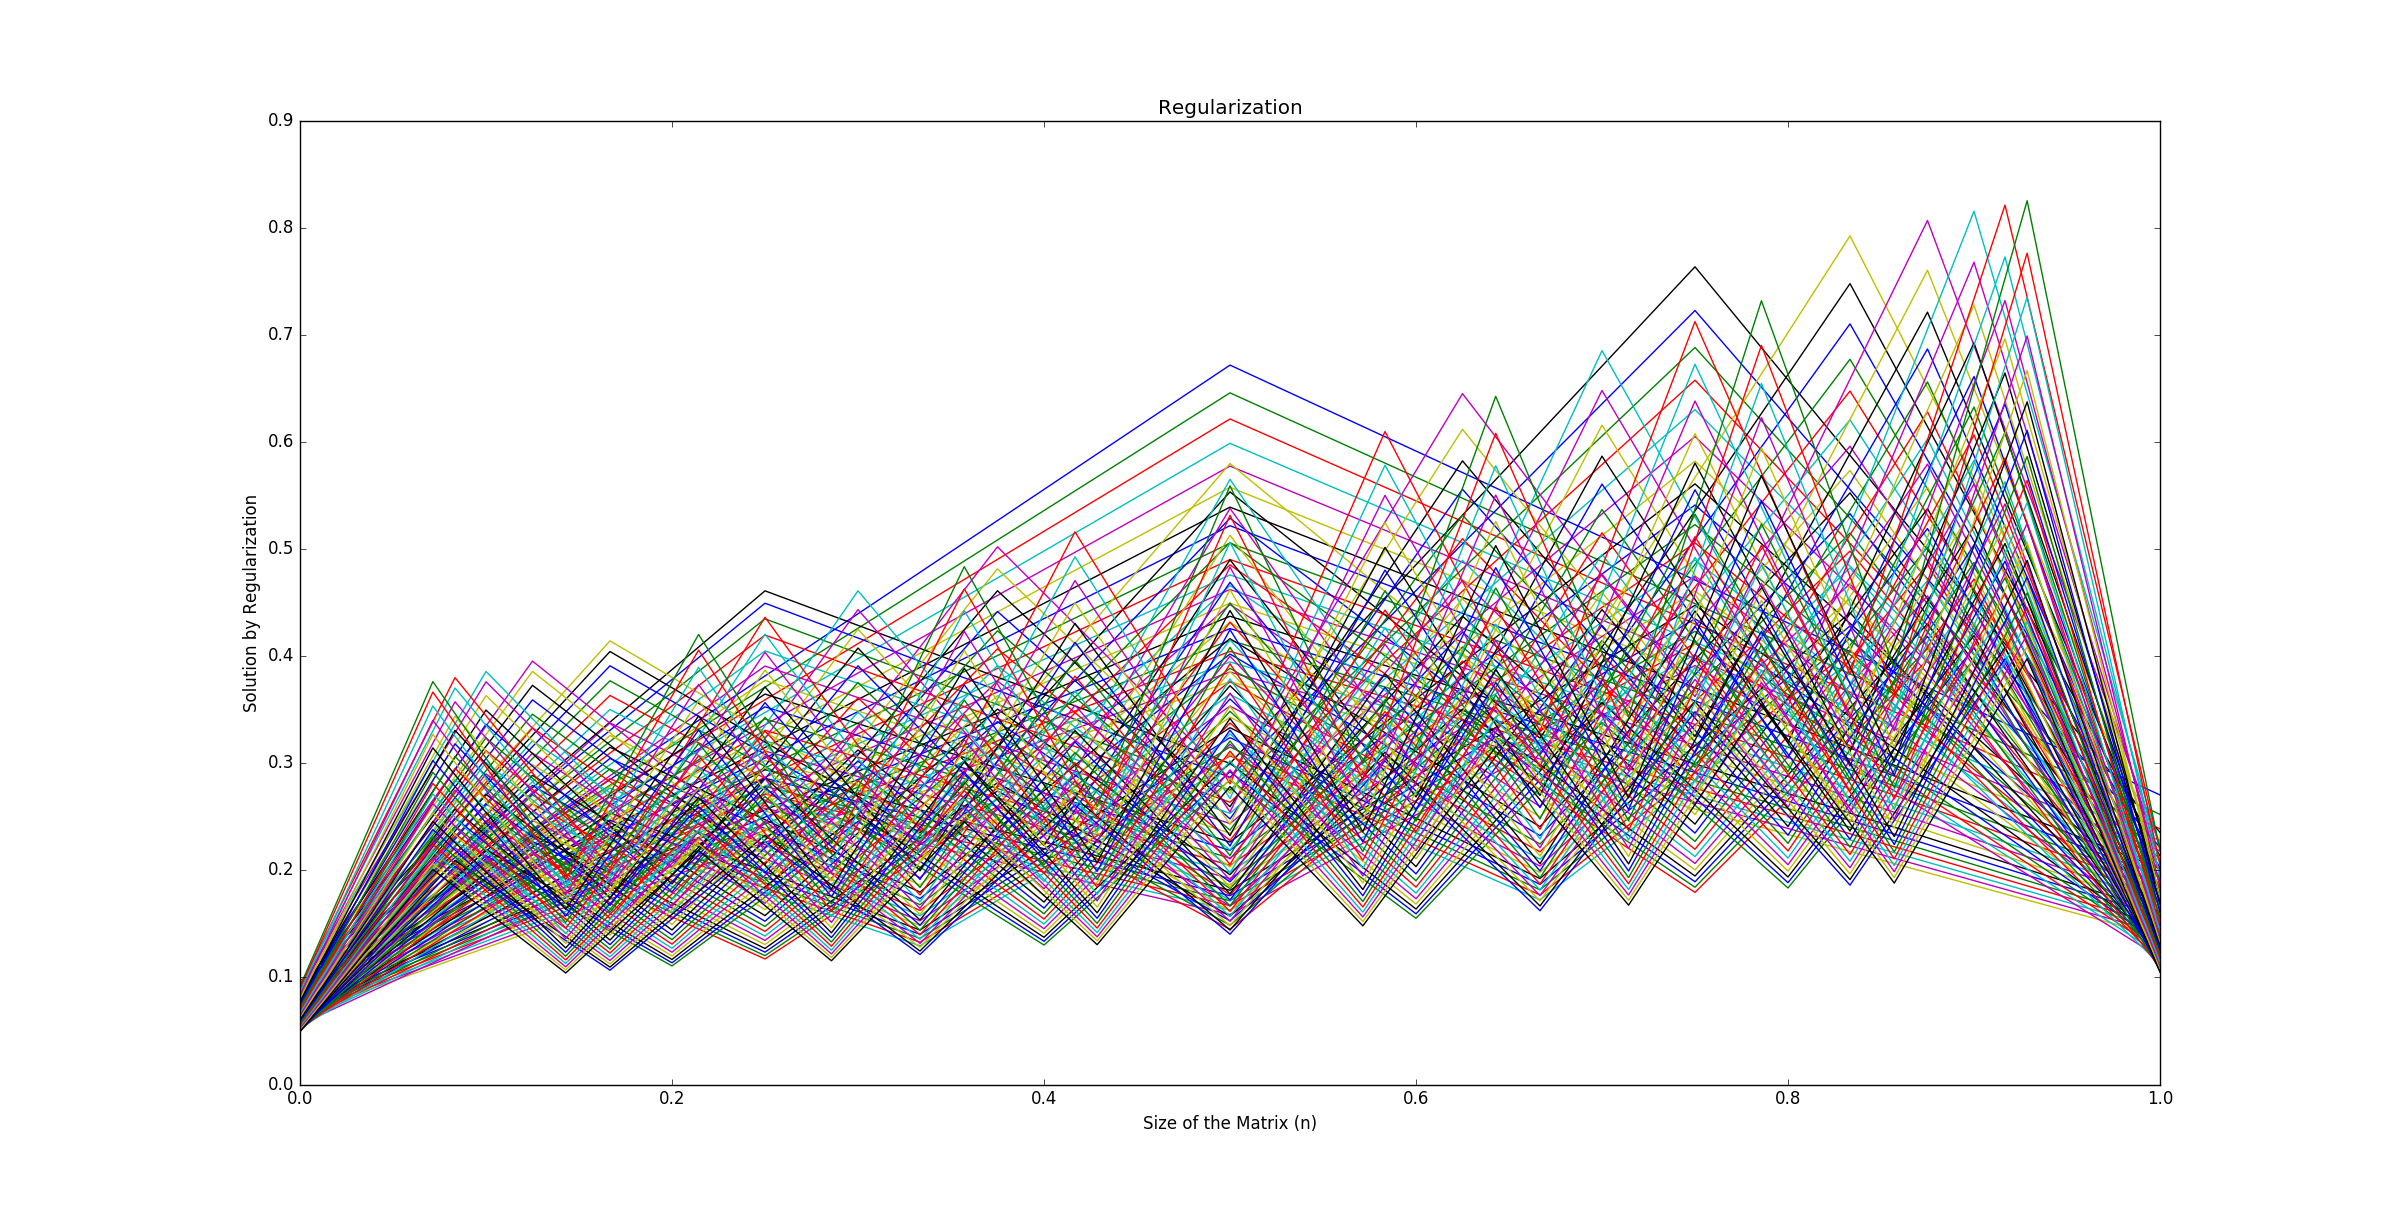
\includegraphics[width = 7in, height = 4in]{RG}
\end{center}
\begin{center}
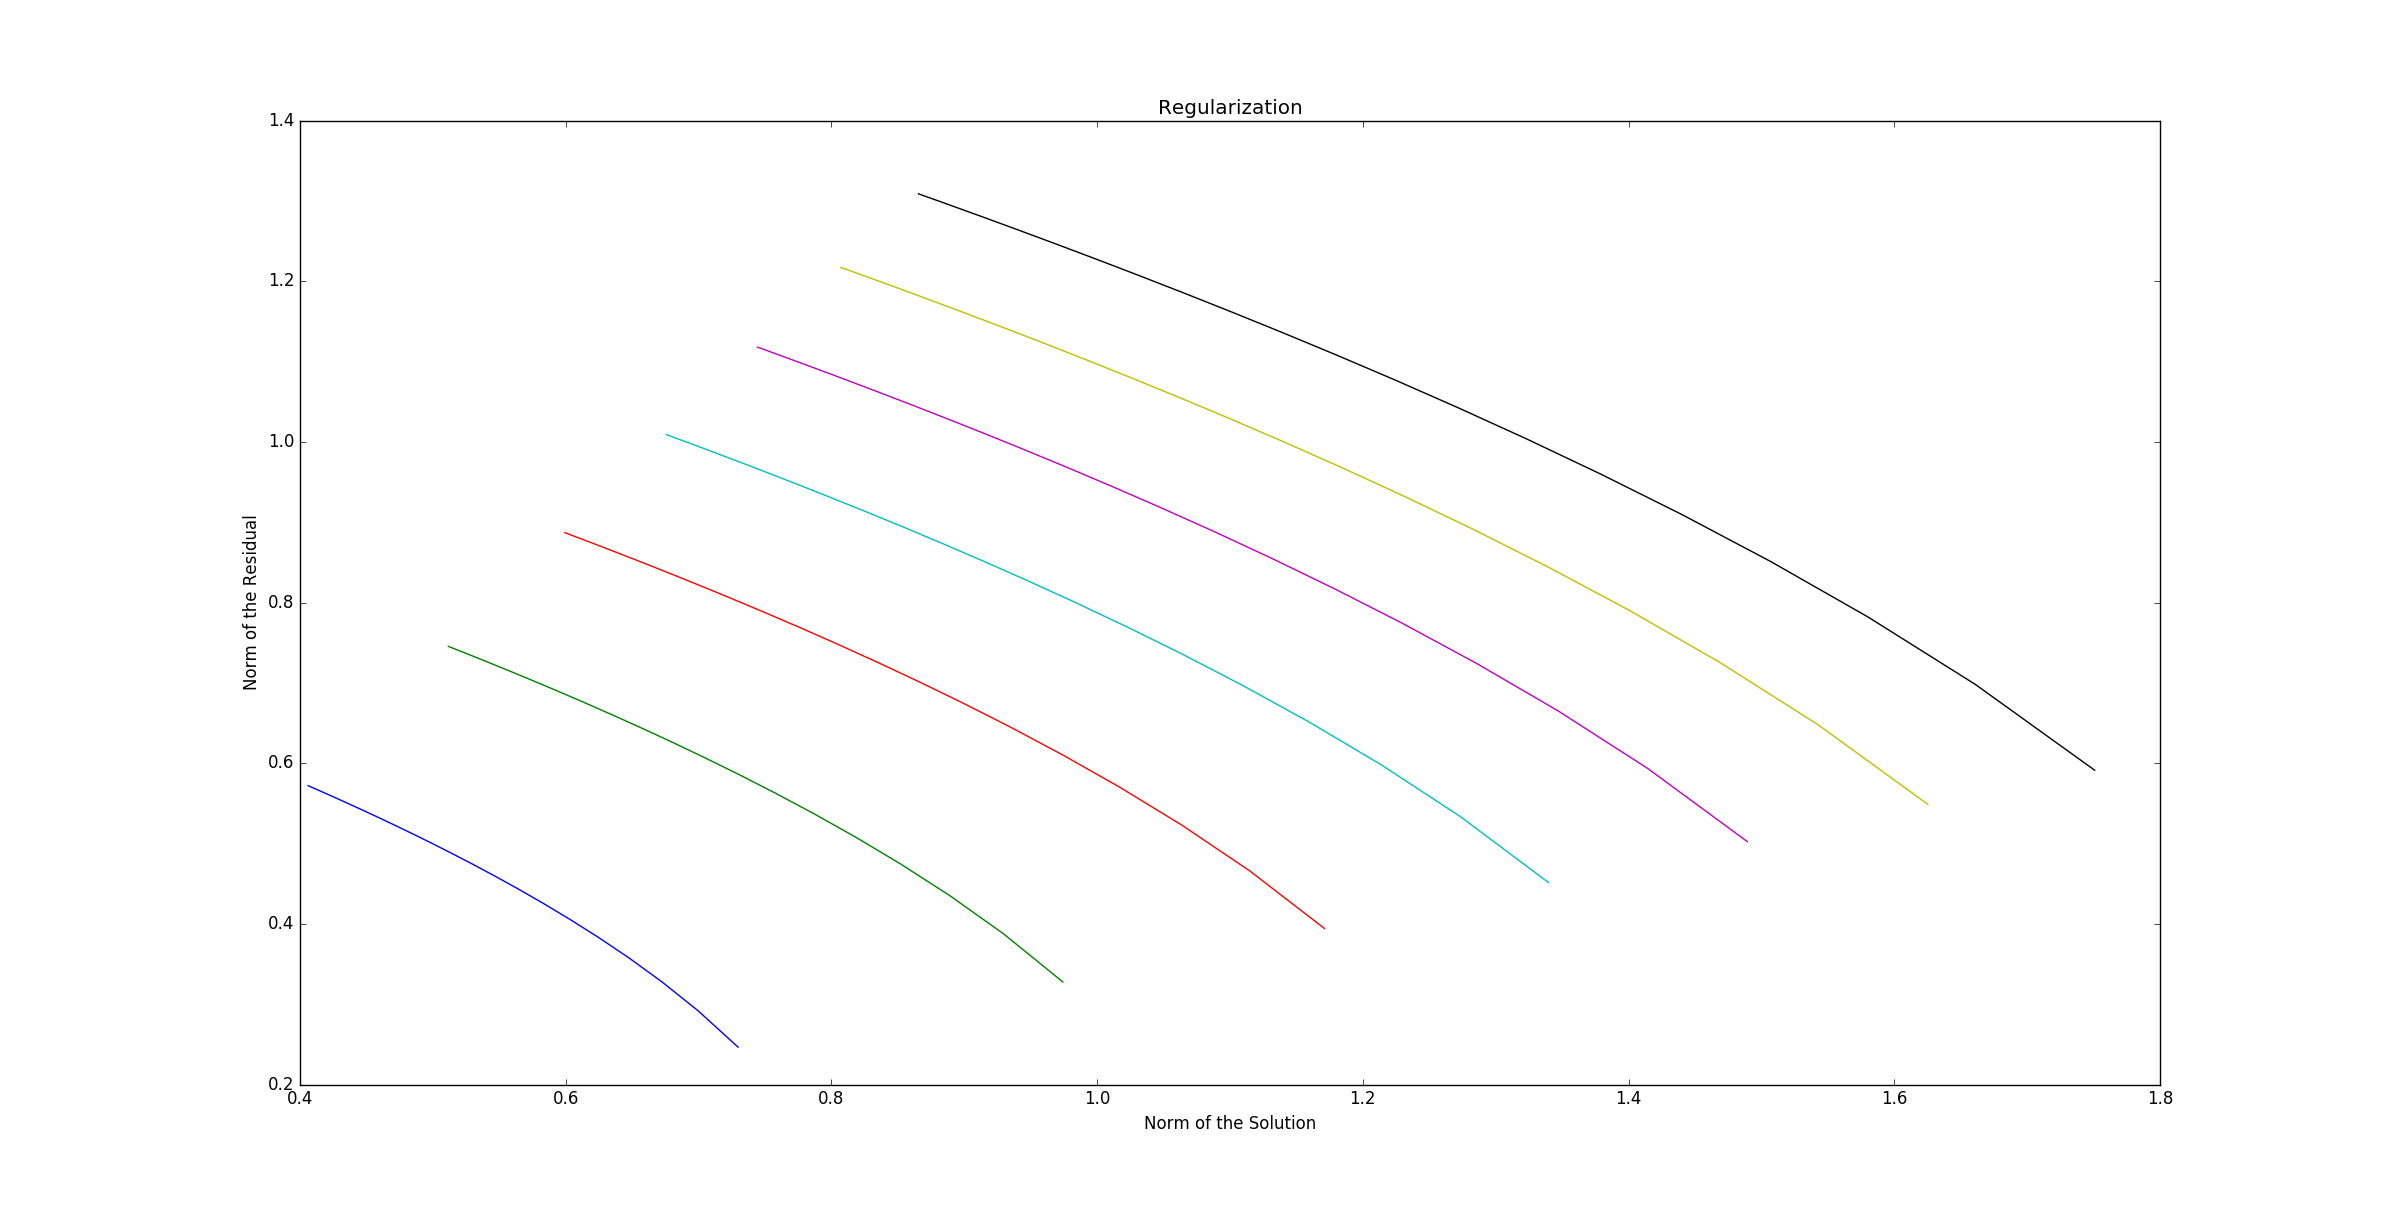
\includegraphics[width = 7in, height = 4in]{NSNR}
\end{center}\hrule
\subsection*{(e) and (f): Constrained and Unconstrained Optimization}
The constrained optimization is the best among all the methods as can be observed by the plots below: 
\begin{center}
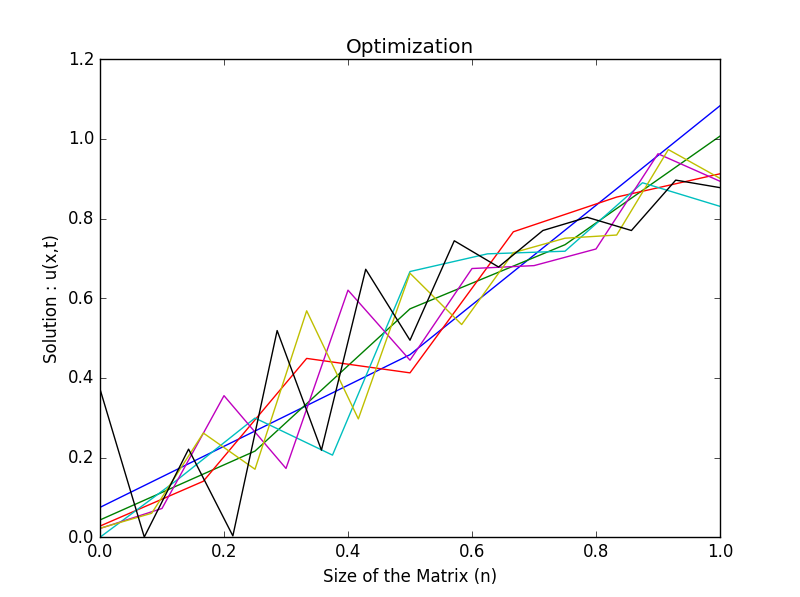
\includegraphics[width = 7in, height = 4in]{OP}
\end{center}
\begin{center}
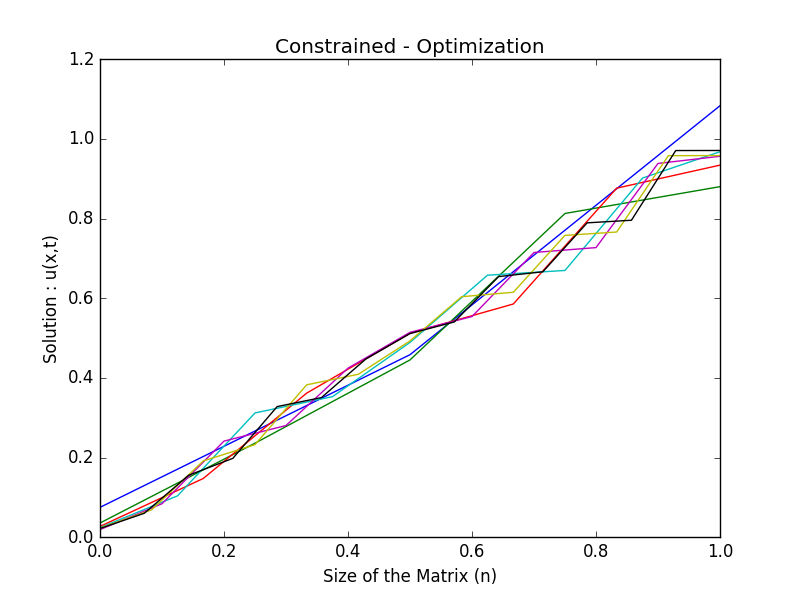
\includegraphics[width = 7in, height = 4in]{CO}
\end{center}\hrule
\section*{Notes: }
\begin{itemize}
\item For regularization the error is damped but it is very large and hence any particular improvement towards the true solution cannot be inferred from the graph. 
\item The Constrained Optimization follows the trendline for the true solution, the closest among all the methods. It is followed by the unconstrained optimization. 
\item The Gaussian Elimination with partial pivoting does not perform satisfactorily because the matrix becomes increasingly ill-conditioned. This is verified by the plot of the conditioning number with the matrix size (n).
\item The solution given by the SVD fluctuate about the true solution (trendline) but the mean values are close to the actual solution. The negative and the positve errors cancel each other in one oscillation. 
\end{itemize}
\newpage\section*{Problem 8.18: Poly-fits and Splines}
The given data points are interpolated through polynomial fits and splines of different types and the corresponding plots are attached below: 
\subsection*{(a): Least Squares Polynomial Fits}
\begin{center}
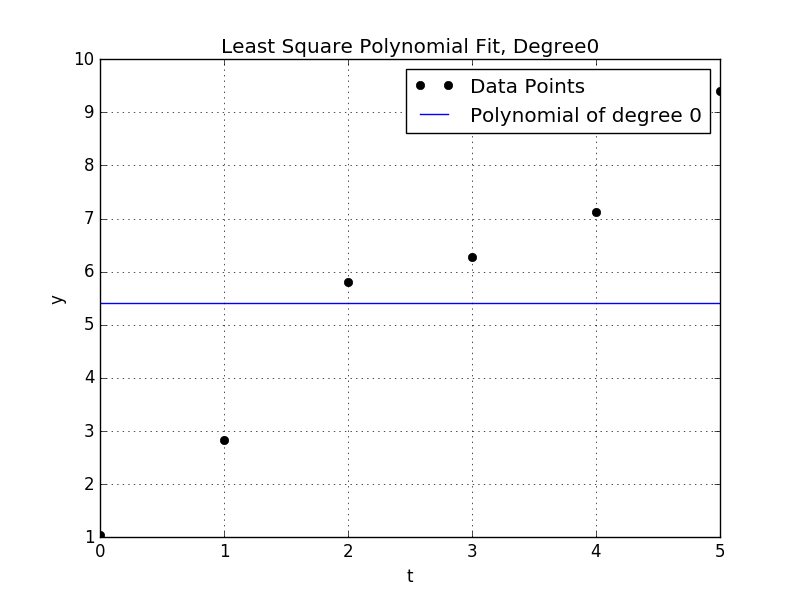
\includegraphics[width = 7in, height = 4in]{Pol0}
\end{center}
\begin{center}
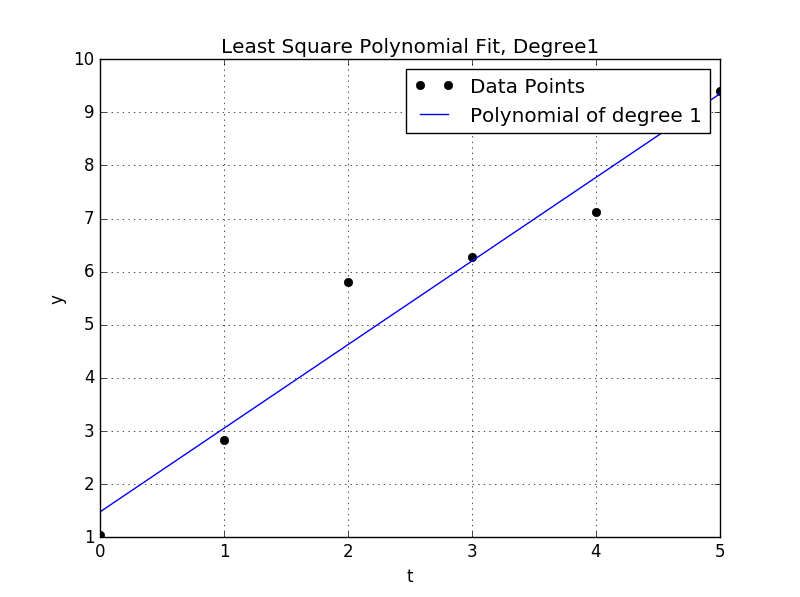
\includegraphics[width = 7in, height = 4in]{Pol1}
\end{center}
\begin{center}
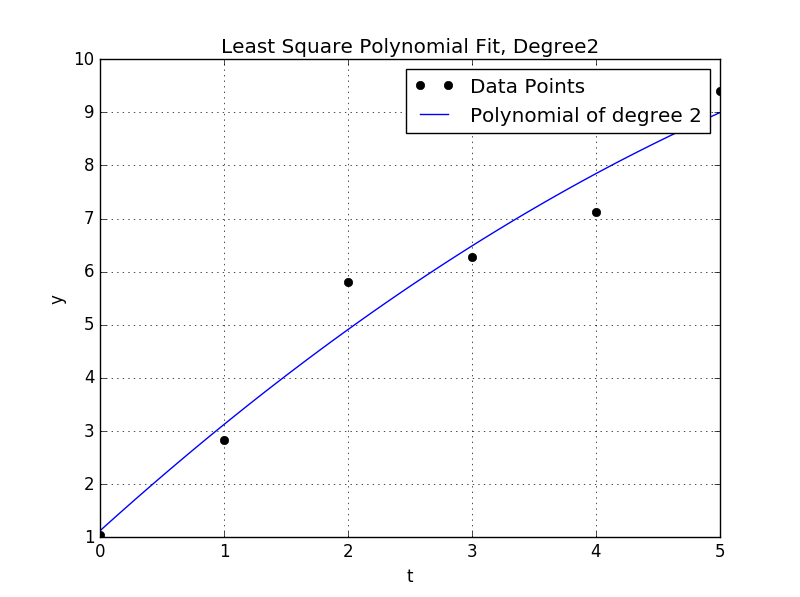
\includegraphics[width = 7in, height = 4in]{Pol2}
\end{center}
\begin{center}
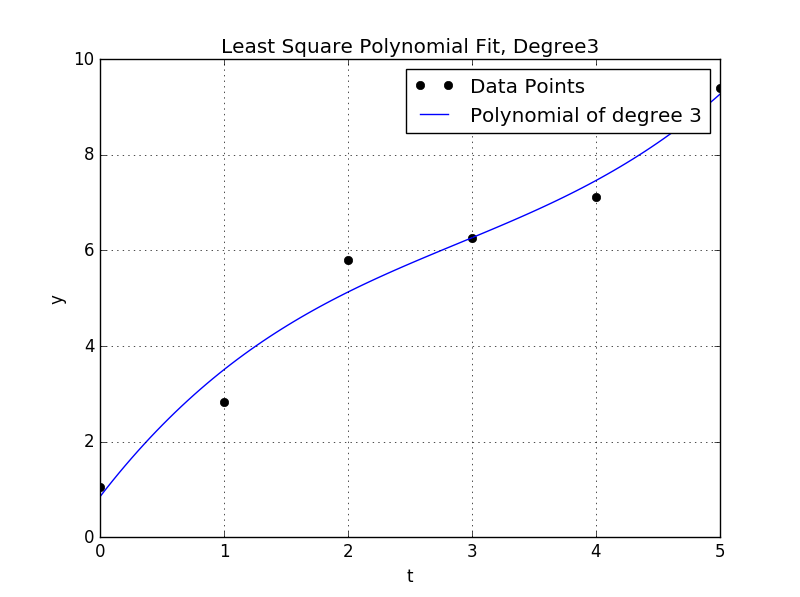
\includegraphics[width = 7in, height = 4in]{Pol3}
\end{center}
\begin{center}
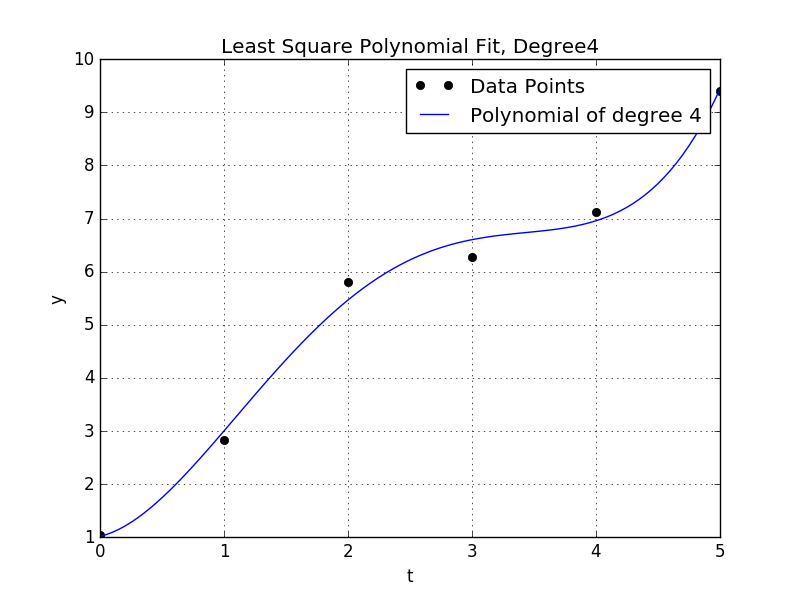
\includegraphics[width = 7in, height = 4in]{Pol4}
\end{center}
\begin{center}
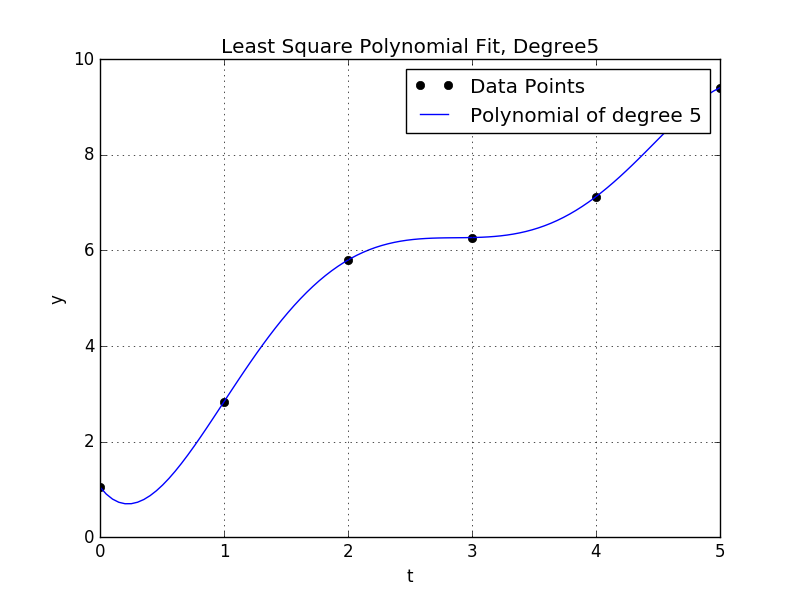
\includegraphics[width = 7in, height = 4in]{Pol5}
\end{center}
\subsection*{(b): Cubic Spline}
\begin{center}
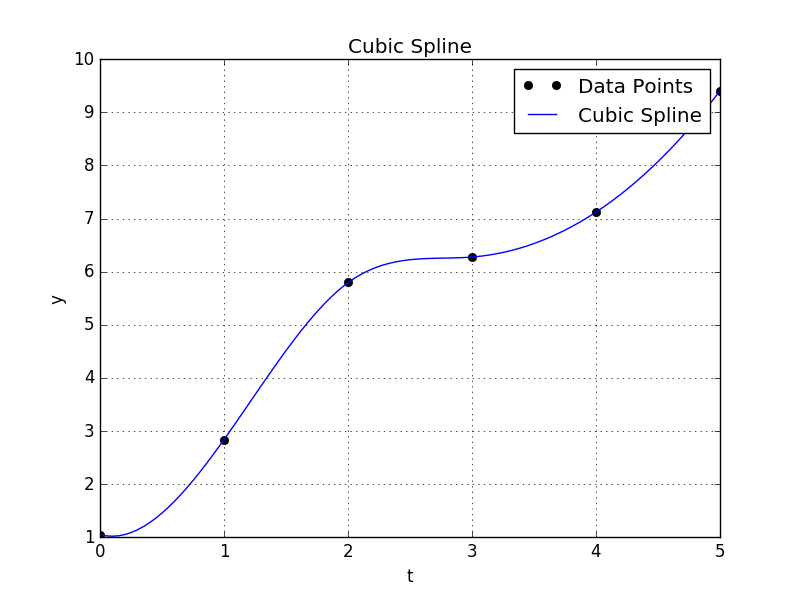
\includegraphics[width = 7in, height = 4in]{CSpl}
\end{center}
\newpage\subsection*{(c): Smoothening Spline of different degrees}
\begin{center}
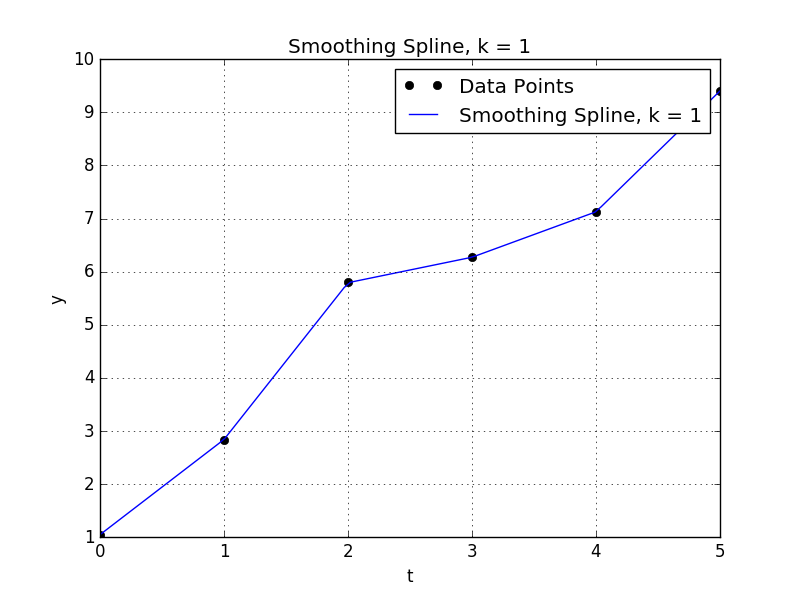
\includegraphics[width = 7in, height = 4in]{SmSpl1}
\end{center}
\begin{center}
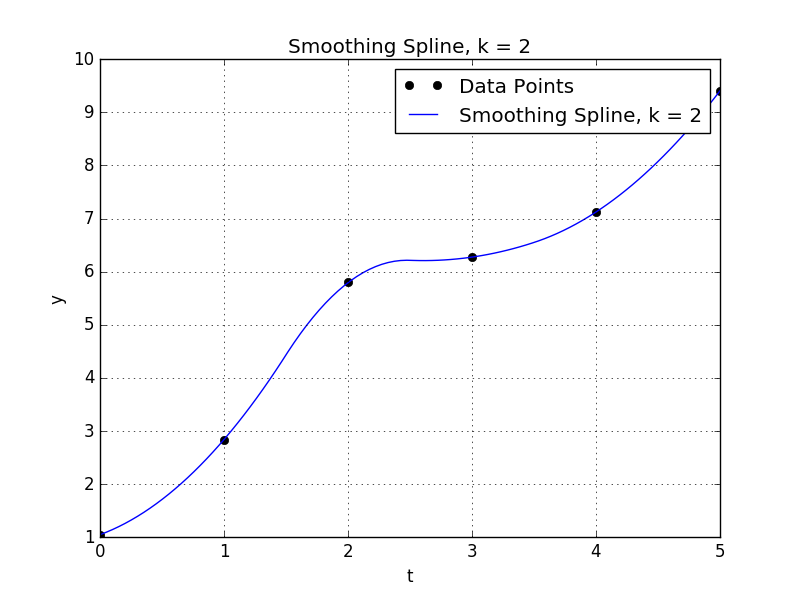
\includegraphics[width = 7in, height = 4in]{SmSpl2}
\end{center}\begin{center}
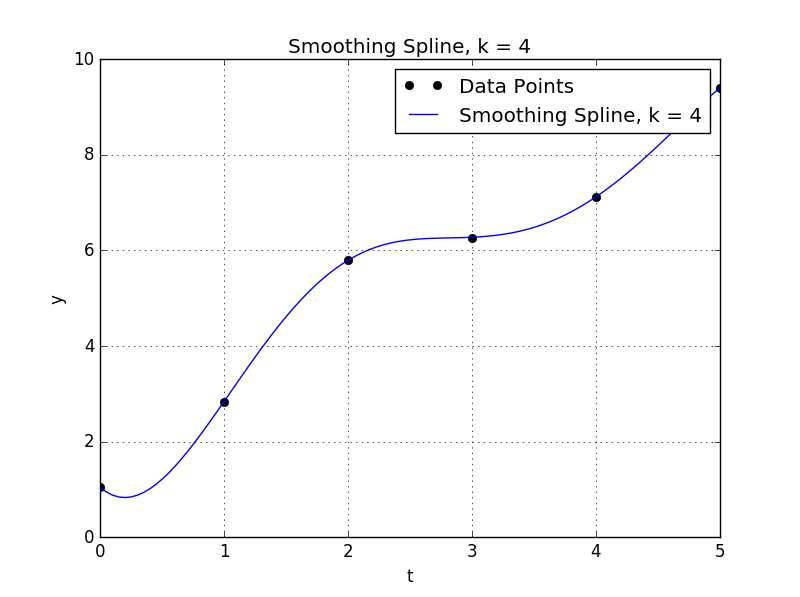
\includegraphics[width = 7in, height = 4in]{SmSpl4}
\end{center}\begin{center}
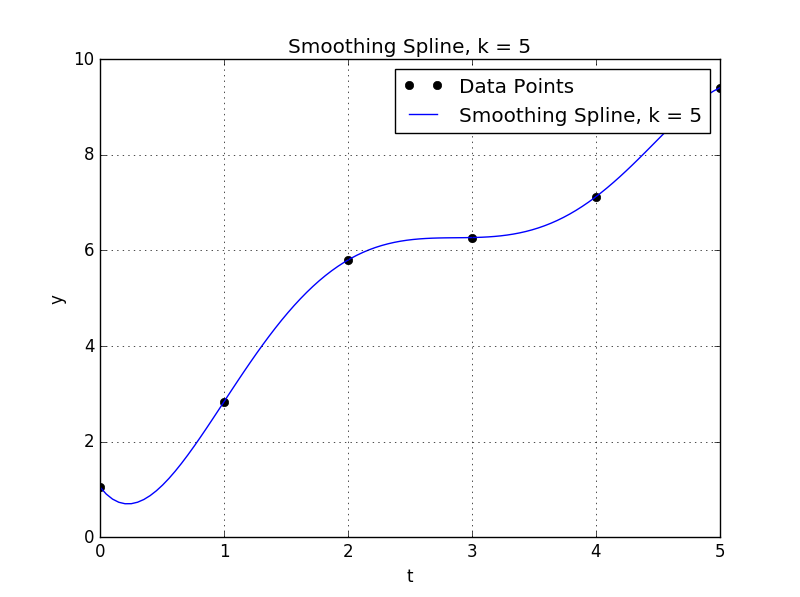
\includegraphics[width = 7in, height = 4in]{SmSpl5}
\end{center}
\newpage\subsection*{(d) Hermite Spline}
\begin{center}
\includegraphics[width = 7in, height = 4in]{HSpl}
\end{center}\hrule
\subsection*{Notes: }
The Splines, in general are better in interpolating the data points smoothly, and also preserving the monotonicity of the data. Hermite Spline follows the trend of the data-set more closely as compared to the cubic-spline. Least Squares Polynomial Interpolants may/maynot pass through the data points always. Also several problems can be incurred (derivatives etc.) when the data set is perturbed.  
\newpage\section*{Appendix: Python Codes}
\subsection*{5.22}
The Python code used to solve the problem 5.22 is appended below: 
\lstinputlisting[language=Python]{522.py}\hrule
\subsection*{5.24}
The code used to solve the problem 5.24 is appended below: 
\lstinputlisting[language=Python]{524.py}\hrule
\subsection*{8.6}
The code used to solve the problem 8.6 is appended below: 
\lstinputlisting[language=Python]{86.py}\hrule
\subsection*{8.10}
The code used to solve the problem 8.10 is appended below: 
\lstinputlisting[language=Python]{810.py}\hrule
\subsection*{8.17}
The code used to solve the problem 8.17 is appended below: 
\lstinputlisting[language=Python]{8.17.py}\hrule
\subsection*{8.18}
The code used to solve the problem 8.18 is appended below: 
\lstinputlisting[language=Python]{8.16.py}\hrule\hrule\hrule
\end{document}